\section{Problema}\label{problema}

Quesito di cui si richieda ad altri o a sé stessi la soluzione, partendo
di solito da elementi noti.

Un problema computazionale: problema risolvibile mediante algoritmi,
espresso in generale come corrispondenza tra input e output.

\subsection{Istanza}\label{istanza}

particolare occorrenza del problema data da una specifica configurazione
degli input

\section{Algoritmo}\label{algoritmo}

\emph{\textbf{\ul{Def:}} Un insieme ordinato di operazioni/istruzioni
elementari, non ambigue, ed effettivamente computabili che, quando
eseguito su certi dati in ingresso (input), produce un risultato
(output) arrestandosi in tempo finito.}

Un modo per risolvere un problema. Esistono due diversi momenti relativi
ad essi:

\begin{itemize}
\item
  specifica / rappresentazione

  \begin{itemize}
  \item
    implementazione: algoritmo rappresentato in forma eseguibile
    (programma)
  \end{itemize}
\item
  esecuzione: un esecutore segue quanto indicato dall'algoritmo su
  un'istanza del problema

  \begin{itemize}
  \item
    L'esecuzione di un algoritmo è il processo di risoluzione del
    problema
  \end{itemize}
\end{itemize}

Più algoritmi possono risolvere lo stesso problema, problema del
confronto e scelta dell'algoritmo migliore, e uno stesso algoritmo può
essere rappresentato in modi diversi.

\textbf{L'informatica} è la disciplina che cerca di fornire il
fondamento scientifico a vari argomenti, \textbf{l'algoritmo} è una
sequenza finita di passi formali (non ambigui ed eseguibili dalla
macchina) che trasformano un input in un output invece un
\textbf{programma} è la rappresentazione di un algoritmo comprensibile
dalla macchina.

\subsection{\texorpdfstring{
Requisiti/proprietà}{ Requisiti/proprietà}}\label{requisitiproprietuxe0}

\begin{itemize}
\item
  \emph{Ordinamento delle operazioni}: un algoritmo dovrebbe avere una
  struttura dove è chiaro l'ordine di esecuzione dei suoi passi.
\item
  \emph{Non ambiguità}: l'esecutore deve poter interpretare le
  istruzioni in modo univoco.
\item
  \emph{Istruzioni effettivamente computabili:} l'esecutore deve essere
  in grado di eseguire le operazioni indicate.
\item
  \emph{Finitezza:} l'algoritmo dovrebbe consistere in un numero finito
  di passi, richiedere un numero finito di input/risorse, e terminare in
  tempo finito.
\end{itemize}

\subsection{Programmazione imperativa}\label{programmazione-imperativa}

In questo stile, gli algoritmi sono espressi come sequenze di istruzioni
che il computer deve eseguire e che modificano lo stato del programma;
coerente con l'architettura di von Neumann e con il modo con cui i
computer funzionano a livello hardware.

Questo tipo di paradigma si concentra sul ``come'' invece che sul
``cosa'' (paradigmi dichiarativi).

\subsection{Caratteristiche}\label{caratteristiche}

\begin{itemize}
\item
  \emph{Correttezza}: un algoritmo è corretto se, per ogni istanza del
  problema, termina con l'output corretto.
\item
  \emph{Generalità}: un algoritmo dovrebbe applicarsi a una tipologia di
  problemi, e non solamente a specifiche istanze.
\item
  \emph{Determinismo}: partendo dagli stessi input, si dovrebbero
  ottenere gli stessi output.
\item
  \emph{Efficienza}: l'esecuzione dell'algoritmo dovrebbe avere un costo
  accettabile.
\end{itemize}

\section{Programmazione strutturata}\label{programmazione-strutturata}

Paradigma di programmazione basato sull'uso di costrutti di controllo
del flusso e blocchi di codice.

\textbf{Teorema di Böhm-Jacopini}: \emph{qualsiasi programma può essere
scritto usando tre tipi di strutture di controllo: sequenza, selezione e
iterazione.}

Si usa lo pseudo codice per astrarre da dettagli specifici dei linguaggi
di programmazione e per semplificare la notazione e migliorare la
leggibilità.

\emph{Non esiste nessuno standard per la sintassi dello pseudocodice,
ognuno può scriverselo come vuole.}

Algoritmi ricorsivi

Un algoritmo viene detto ricorsivo quando nel suo corpo richiama se
stesso.

\textbf{Principio di induzione:}

\emph{Data una proprietà P. Se P(0) è vera e P(n) ⇒ P(n + 1) per ogni n,
allora P(n) è vera per ogni n.}

\emph{(∀P){[}P(0) ∧ (∀k ∈ N)(P(k) ⇒ P(k + 1)){]} ⇒ (∀n ∈ N){[}P(n){]}}

Principio per dimostrazioni:

\begin{enumerate}
\def\labelenumi{\arabic{enumi}.}
\item
  \emph{caso base}: si dimostra che P(0) o P(1) è vera
\item
  \emph{passo induttivo}: assumendo P(n) vera, si dimostra che anche P(n
  + 1) lo è
\end{enumerate}

\section{Funzioni ricorsive}\label{funzioni-ricorsive}

Una funzione ricorsiva corretta ha le seguenti caratteristiche:

\begin{itemize}
\item
  include uno o più casi base in cui il valore della funzione viene
  calcolato senza invocazione ricorsiva;
\item
  includa una o più invocazioni ricorsive della funzione, tipicamente
  con argomenti che progressivamente ``avvicinano'' ai casi base.
\end{itemize}

\section{Divide-et-impera}\label{divide-et-impera}

Con questa tecnica dividiamo il problema in sottoproblemi più facili e
li risolviamo uno a uno e li combiniamo insieme per risolvere il
problema iniziale.

\emph{Nella creazione di un algoritmo ricorsivo bisogna pensare prima al
caso base e successivamente al passo della ricorsione}

\section{Tipi di ricorsione}\label{tipi-di-ricorsione}

\begin{enumerate}
\def\labelenumi{\arabic{enumi}.}
\item
  \textbf{Diretta}: la procedura richiama direttamente se stessa;
\item
  \textbf{Indiretta}: la procedura invoca un'altra procedura che
  richiama (direttamente o indirettamente) la procedura originaria;
\item
  \textbf{Lineare:} la procedura include una sola chiamata ricorsiva
  (es. fattoriale);
\item
  \textbf{Multipla}: la procedura include più di una chiamata ricorsiva
  (es. Fibonacci) se ci sono solo due chiamate è detta \emph{binaria};
\item
  \textbf{Mutua}: caso particolare di ricorsione indiretta dove la
  procedura A chiama una procedura B che chiama nuovamente la procedura
  A in modo diretto (es. pari/dispari);
\item
  \textbf{Coda}: caso particolare di ricorsione lineare in cui la
  chiamata ricorsiva è l'ultima istruzione della procedura;
\item
  \textbf{Annidata (innestata)}: la chiamata ricorsiva ha come argomento
  un'ulteriore chiamata ricorsiva (es. funzione di Ackermann);
\item
  \textbf{Infinita}: : quando non vi è (riduzione del problema che porta
  a) caso base gestito senza ricorsione.
\end{enumerate}

\subsection{Esempi}\label{esempi}

Lineare:

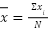
\includegraphics[width=5.08854in,height=2.17909in]{media/image54.png}

Multipla

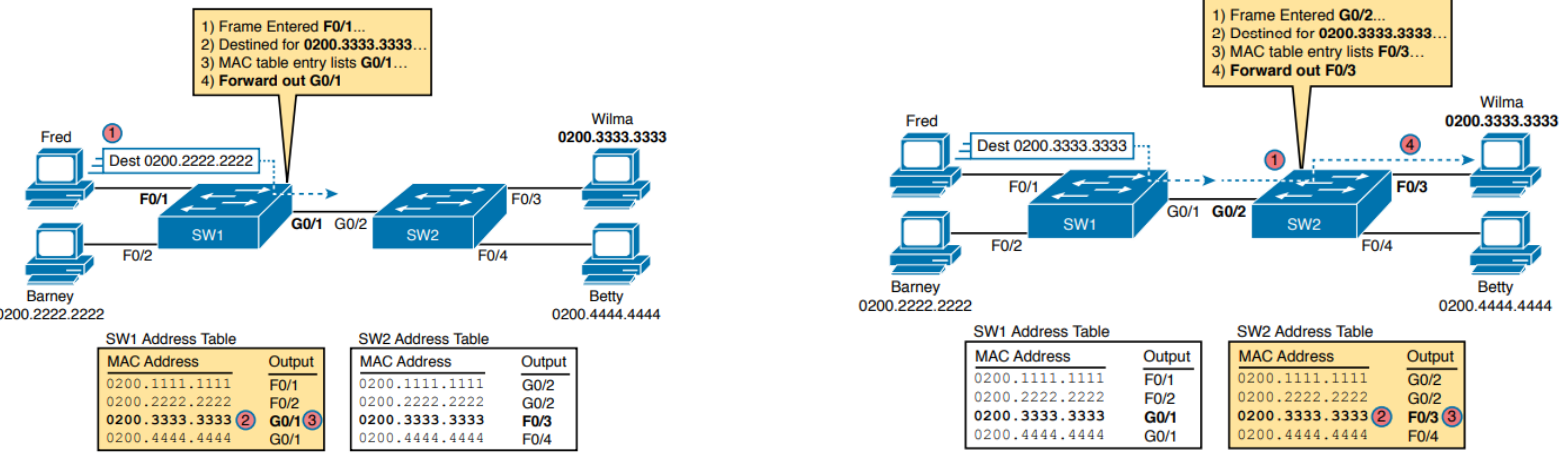
\includegraphics[width=6.26772in,height=1.59722in]{media/image63.png}

Mutua

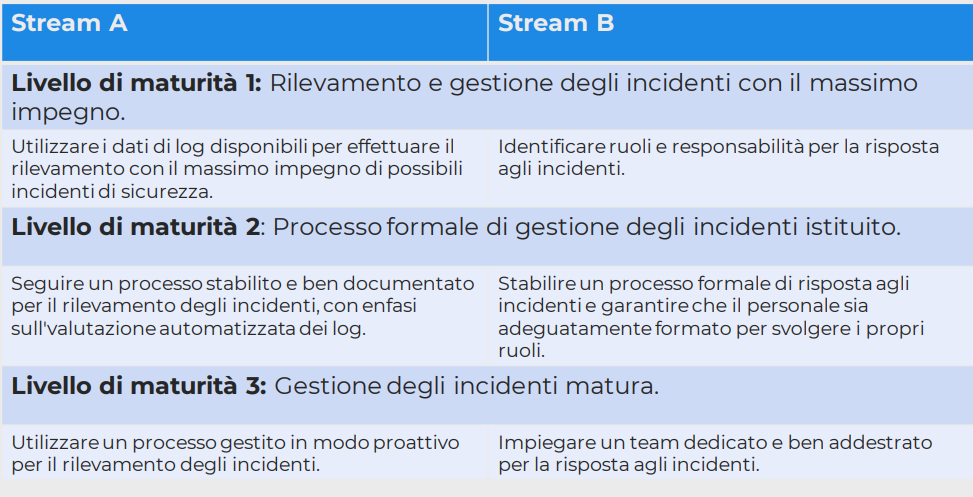
\includegraphics[width=6.26772in,height=1.36111in]{media/image74.png}

Efficienza degli algoritmi

Caratterizzare l'efficienza è un aspetto importante dell'analisi e
progettazione di algoritmi, esistono due nozioni fondamentali:

\begin{itemize}
\item
  efficienza in tempo
\item
  efficienza in spazio
\end{itemize}

\section{Tempi di esecuzione}\label{tempi-di-esecuzione}

τ (Tau) è la funzione che serve per identificare il tempo di esecuzione,
determinata dalla natura e struttura dell'algoritmo.

La τ dipende dalla dimensione n dell'input, dalle istanze dell'input (se
dobbiamo valutare un algoritmo di ordinamento il modo in cui l'array ci
arriva è essenziale) e dall'esecutore.

In sostanza:

\emph{\textbf{`\,'}La variazione del tempo d'esecuzione al variare della
dimensione n dell'input può essere caratterizzata da una funzione τ
(n)\textbf{`\,'}}

Alcune forme frequenti di τ(n) sono:

\begin{itemize}
\item
  \textbf{meno che lineare:} \(\log_{e}(n),\log_{2}(n),\ \ \)
  --\textgreater{} all'aumento di n il tempo di esecuzione aumenta
  lentamente
\item
  \textbf{lineare}: \(k \cdot \ n\)
\item
  \textbf{più che lineare}:
  \({n*log(n),\ n}^{k}(polinomiale),\ k^{n}(esponenziale),\ n!,\ n^{n}\)
  --\textgreater{} all'aumento di n il tempo di esecuzione aumenta
  velocemente
\end{itemize}

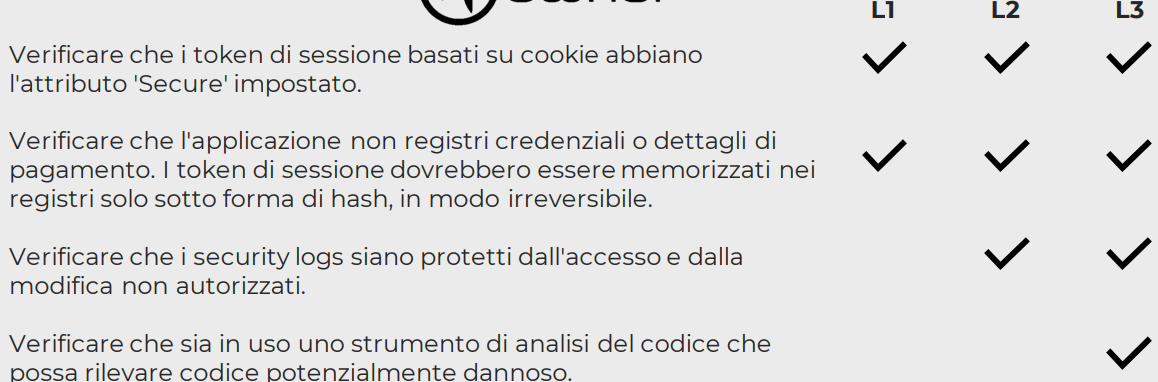
\includegraphics[width=6.26772in,height=4.55556in]{media/image64.png}

Per una dimensione n esistono tre casi:

\begin{enumerate}
\def\labelenumi{\arabic{enumi}.}
\item
  \textbf{Best case}: le configurazioni della struttura dati di ingresso
  \(d\) che danno luogo al tempo minimo;
\item
  \textbf{Average case}: le configurazioni della struttura dati di
  ingresso \(d\) ritenute ``normali'' (e.g., più frequenti in pratica);
\item
  \textbf{Worst case}: le configurazioni della struttura dati di
  ingresso \(d\) che danno luogo al tempo massimo.
\end{enumerate}

La prima casistica non è rilevante, invece:

\begin{itemize}
\item
  la \emph{complessità worst-case} serve per capire i limiti di
  applicabilità pratica permettendo di fare ragionamenti sulla safety
  (controlli real-time);
\item
  la \emph{complessità average-case} è difficile da valutare essendo non
  semplice caratterizzare input tipici.
\end{itemize}

\section{Andamento asintotico}\label{andamento-asintotico}

Essendo che τ(n) è influenzato dal hardware o dal linguaggio di
programmazione si vuole astrarre da questi aspetti, infatti non ci
interessa quanto tempo ci mette un determinato computer rispetto ad un
altro ma bisogna capire l'andamento del tempo asintoticamente quindi al
crescere dell'input.

Anche con tre tempi di esecuzione differenti (essendo fatti su hardware
diversi) essi potrebbero essere accomunati dallo stesso andamento.

\section{Modello di calcolo}\label{modello-di-calcolo}

Durante lo studio degli algoritmi si considera un modello di calcolo
standard chiamato \textbf{RAM} \emph{(Random Access Machine)}, cioè un
sistema mono-processore (istruzioni in sequenza) dove le istruzioni
semplici richiedono tempo costante.

Con \(T(n)\) denotiamo il tempo stimato per l'esecuzione dell'algoritmo
nella RAM (stima tempo effettivo τ(n)).

\section{\texorpdfstring{Complessità computazionale
}{Complessità computazionale }}\label{complessituxe0-computazionale}

È l'ordine di grandezza della funzione T(n)

\section{Ordini di infiniti}\label{ordini-di-infiniti}

Una funzione \(f(n)\) tale che \(\lim_{n \rightarrow c}f(n) = \infty\) è
infinita per \(n\  \rightarrow \ c\).

Due funzioni \(f(n)\) e \(g(n)\) sono \textbf{infiniti simultanei} se
entrambe sono infinite per \(n\  \rightarrow \ c\).

Quindi se abbiamo funzioni con dei tempi di esecuzione \(nlog(n)\) o
\(n^{3}\) con \(n\) che tende all'infinito avremo solo funzioni tendenti
ad esso e non saremo in grado di capire quale ha tempi di esecuzione
migliori. Quindi per confrontare diversi infiniti dobbiamo determinare
quale ``\emph{tende all\textquotesingle infinito più rapidamente}''
andando a studiare il limite del rapporto \(\infty/\infty\) (forma
indeterminata).

Le casistiche sono:

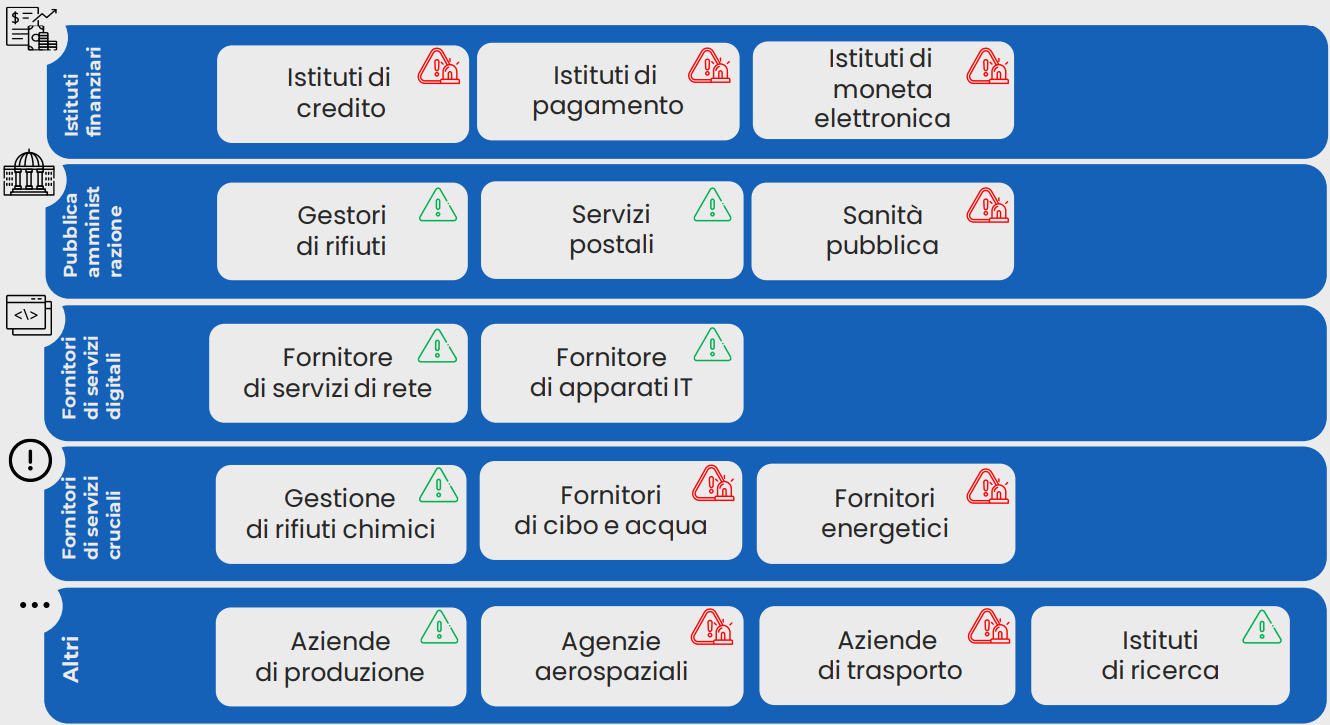
\includegraphics[width=4.34401in,height=1.78234in]{media/image60.png}

\section{Analisi asintotica}\label{analisi-asintotica}

Abbiamo capito che il tasso di crescita del tempo stimato di esecuzione
T(n) di un algoritmo da una semplice caratterizzazione della relativa
efficienza e calcolare il tempo esatto non serve visto che per input
grandi le costanti moltiplicative e i termini di ordine inferiore del
tempo effettivo di esecuzione sono trascurabili ed solo la forma della
funzione di n che definisce l'andamento.

\textbf{Efficienza asintotica \textbar{} Def:}

\emph{È quella che si studia per dimensioni di n tali per cui solo
l'ordine del tasso di crescita è rilevante}

\textbf{Tempo di esecuzione asintotico \textbar{} Def:}

\emph{Approssimazione del tempo d'esecuzione di un algoritmo mediante
una ``più semplice'' funzione di simile ordine di crescita}

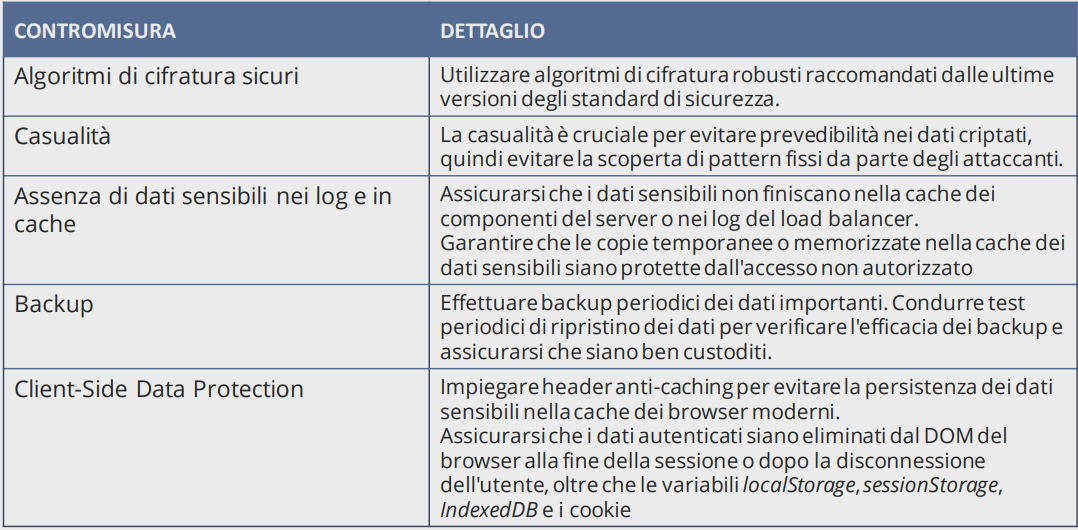
\includegraphics[width=3.82686in,height=2.84896in]{media/image51.png}

\subsection{Notazione asintotica}\label{notazione-asintotica}

Notazione standard per caratterizzare l'efficienza in tempo di un
algoritmo

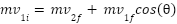
\includegraphics[width=4.48053in,height=1.52604in]{media/image35.png}

Si suddividono in altre 3 notazioni che sono:

\begin{itemize}
\item
  \(O\) \textbf{{[}O-grande{]}}: data una funzione (di confronto)
  \(g(n)\):
\end{itemize}

\begin{quote}
\(O(g(n))\) individua tutte le funzioni \(f(n)\) tale per cui esiste una
costante reale maggiore di 0 (\(c\), \(n_{0}\)) tale per cui questa
condizione è verificata:
\(0 \leq f(n) \leq c \cdot g(n),\forall n \geq n_{0}\) \emph{(}\(f(n)\)
\emph{compresa tra 0 e} \(c \cdot g(n)\) \emph{per tutti i valori di}
\(n > n_{0}\)\emph{).}

Quindi possiamo individuare un certo valore \(n_{0}\) di dimensioni del
problema e una certa costante moltiplicativa tale per cui dal punto
\(n_{0}\) individuato, la funzione \(g(n)\) (moltiplicata per un fattore
a scelta) va a dominare dall'alto la nostra funzione.

In sostanza:

\(g(n)\) \emph{è un limite superiore o upper bound asintotico per}
\(f(n)\)

\emph{e}

\(f(n)\) \emph{asintoticamente cresce come o meno di} \(g(n)\)

\textbf{Esempio:}

Dimostrare che \(n^{2} \in O(n^{3})\)

\(\downarrow\) \(\  \downarrow\)

\(\ f(n)\ \ \ \ \ \ \ \ \ \ g(n)\ \ \)

Dobbiamo usare la definizione di \(O\)\textbf{,} quindi esiste una
costante \(c,\)\(n_{0}\) tale per cui \(f(n)\) è maggiorata da
\(c \cdot g(n)\) e questa cosa è valida per ogni
\(n \geq n_{0}\)\emph{.}

Applichiamo la disequazione che la formula ci da:

\(0 \leq f(n) \leq cg(n)\) \(\Rightarrow\)
\(0 \leq n^{2} \leq c \cdot n^{3}\)

\(\Downarrow\)

\(0 \leq 1 \leq c \cdot n\) \(\Rightarrow\) \(c \geq \frac{1}{n}\)
\end{quote}

\begin{itemize}
\item
  \(\Omega\) \textbf{{[}Omega-grande{]}}: data una funzione \(g(n)\):
\end{itemize}

\begin{quote}
\(\Omega(g(n))\) individua tutte le funzioni \(f(n)\) tale per cui
esiste una costante reale maggiore di 0 (\(c\), \(n_{0}\)) tale per cui
questa condizione è verificata:

\(0 \leq g(n) \leq f(n),\forall n \geq n_{0}\) \emph{(}\(g(n)\)
\emph{compresa tra 0 e} \(f(n)\) \emph{per tutti i valori di}
\(n > n_{0}\)\emph{).}

In sostanza:

\(g(n)\) \emph{è un limite inferiore o lower bound asintotico per}
\(f(n)\)

\emph{e}

\(f(n)\) \emph{asintoticamente cresce come o più di} \(g(n)\)
\end{quote}

\begin{itemize}
\item
  \(\Theta\) \textbf{{[}Theta-grande{]}}: data una funzione \(g(n)\):
\end{itemize}

\begin{quote}
\(\Theta(g(n))\) individua tutte le funzioni \(f(n)\) tale per cui
esiste una costante reale maggiore di 0 (\(c_{1}\),\(c_{2}\), \(n_{0}\))
tale per cui questa condizione è verificata:

\(0 \leq c_{1} \cdot g(n) \leq f(n) \leq c_{2} \cdot g(n),\forall n \geq n_{0}\)

Quindi \(f(n)\) da un certo punto in poi (\(n_{0}\)) è compresa tra
\(c_{1} \cdot g(n)\) e \(c_{2} \cdot g(n)\)

In sostanza:

\(g(n)\) \emph{è un limite asintotico stretto o tight bound per}
\(f(n)\)

\emph{e}

\(g(n)\) \emph{e} \(f(n)\) \emph{hanno lo stesso ordine di grandezza}

\textbf{NB}: \hl{se} \(f(n)\) \hl{appartiene a \textbf{O-grande} di}
\(n^{2}\) \hl{allora sicuramente apparterrà anche a \textbf{O-grande}}
\(n^{3}\), se invece \(f(n)\) appartiene a \textbf{Theta-grande} di
\(n^{2}\) sicuramente \emph{\ul{non}} apparterrà ne a
\textbf{Theta-grande} di \(n\) ne a \textbf{Theta-grande} di \(n^{3}\) .
\end{quote}

\subsubsection{Proprietà e
osservazioni}\label{proprietuxe0-e-osservazioni}

\begin{itemize}
\item
  \textbf{Relazioni}: una funzione \(f\) appartiene a \(\Theta(g(n)\))
  se solo se la funzione appartiene anche a \(O(g(n))\) e
  \(\Omega(g(n))\);
\item
  \textbf{Regola della somma:} se una funzione \(T(n)\) appartiene a
  \(\Theta(f(n)) + \Theta(g(n))\) allora possiamo semplificare
  considerando Theta-grande come il massimo delle due funzioni
  {[}\(\Theta(max(f(n),g(n)))\){]};
\item
  \textbf{I termini di grado inferiore non interessano}: se abbiamo
  \(T(n) = n^{3} + 999n^{2}\) ci interessa valutare solo quello con il
  grado maggiore, essendo gli altri ``contenuti'' in esso;
\end{itemize}

\section{Complessità costrutti}\label{complessituxe0-costrutti}

Per ogni costrutto semplice abbiamo le seguenti complessità:

\begin{itemize}
\item
  \textbf{Istruzioni semplici\emph{: }}qui ci sono assegnamenti e
  operazioni aritmetiche/logiche/relazionali; tutti hanno \(\Theta(1)\).
\item
  \textbf{Sequenza di istruzioni semplici}: uguale a sopra
  (\(\Theta(1)\)).
\item
  \textbf{Costrutti selettivi}: con condizione pari a \(\Theta(1)\):

  \begin{itemize}
  \item
    \(O(max(T_{then},T_{else}))\);
  \item
    \(\Omega(min(T_{then},T_{else}))\);
  \item
    Caso peggiore: \(\Theta(max(T_{then},T_{else}))\);
  \item
    Caso maggiore: \(\Theta(min(T_{then},T_{else}))\).
  \end{itemize}
\item
  \textbf{Costrutti iterativi}:

  \begin{itemize}
  \item
    \emph{for} per \(k(n)\) iterazioni e contando che
    \(T_{init} = T_{cond} = T_{inc} = O(1)\)

    \begin{itemize}
    \item
      \(O(T_{init} + k(n) \cdot (T_{cond} + T_{body} + T_{inc}) + T_{cond}) = O(k(n)T_{body})\);
    \item
      \(\Omega(T_{init} + k(n) \cdot (T_{cond} + T_{body} + T_{inc}) + T_{cond}) = \Omega(k(n)T_{body})\);
    \item
      Caso peggiore: \(\Theta({k_{worst}(n)}_{}T_{body,worst})\);
    \item
      Caso maggiore: \(\ \Theta({k_{best}(n)}_{}T_{body,best})\).
    \end{itemize}
  \item
    \emph{while} e in funzione del numero min e max di iterazioni
    (\(k_{\min}\),\(k_{\max}\))

    \begin{itemize}
    \item
      \(O(k_{\max}T_{body})\) e \(\Omega(k_{\min}T_{body})\);
    \item
      Caso peggiore: \(\Theta({k_{\max} \cdot}_{}T_{body,worst})\);
    \item
      Caso maggiore: \(\ \Theta({k_{\min} \cdot}_{}T_{body,best})\).
    \end{itemize}
  \end{itemize}
\end{itemize}

\subsection{Esempio}\label{esempio}

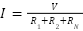
\includegraphics[width=6.26772in,height=3.59722in]{media/image47.png}

Ricorrenze

Il modo di calcolare la complessità degli algoritmi visto
precedentemente non è applicabile alle funzioni ricorsive, infatti per
calcolare la complessità, dobbiamo considerare anche il costo della
chiamata ricorsiva andando a ottenere \textbf{equazioni ricorrenti}.

Ora distinguiamo due contributi:

\begin{itemize}
\item
  \(f(n)\): tempo di tutte le istruzioni che \emph{\textbf{non}
  contengono} chiamate ricorsive;
\item
  \(T(k)\): tempo derivante dalle chiamate ricorsive, invocate su k
  \textless{} n (istanze più piccole del problema---cf.
  divide-et-impera).
\end{itemize}

\section{Metodi di risoluzione delle
ricorrenze}\label{metodi-di-risoluzione-delle-ricorrenze}

Esistono tre metodi principali:

\begin{enumerate}
\def\labelenumi{\arabic{enumi}.}
\item
  \textbf{Metodo iterativo:} si espande l'equazione fino ad arrivare a
  una espressione in funzione di \(n\) e costanti;
\end{enumerate}

\begin{quote}
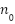
\includegraphics[width=5.25886in,height=3.52467in]{media/image17.png}

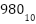
\includegraphics[width=5.30466in,height=3.29023in]{media/image32.png}
\end{quote}

\begin{enumerate}
\def\labelenumi{\arabic{enumi}.}
\setcounter{enumi}{1}
\item
  \textbf{Metodo della sostituzione}: in questo caso: \(T(n)\)
  appartiene a \(O(f(n))\) quindi si effettua un ``guess'' sulla
  possibile soluzione e si utilizza l'induzione matematica per
  dimostrare la correttezza della soluzione;
\end{enumerate}

\begin{quote}
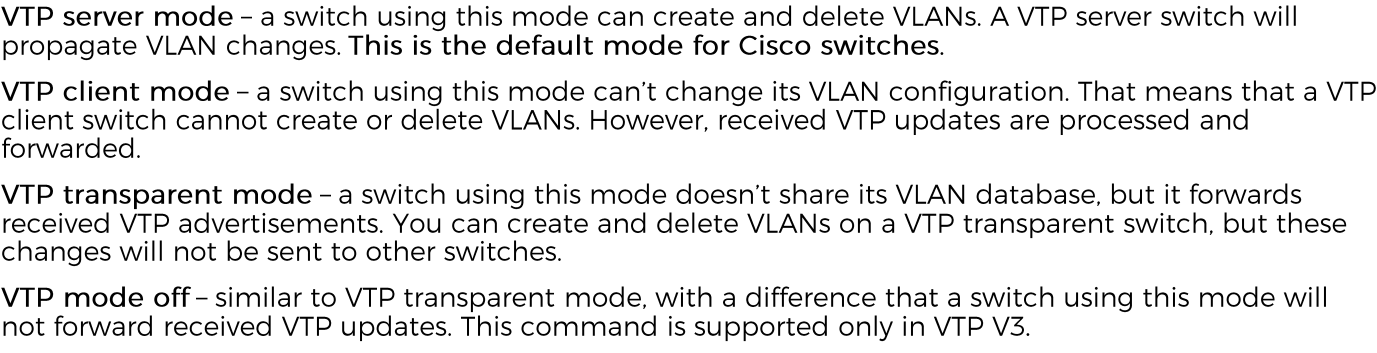
\includegraphics[width=5.07646in,height=2.4539in]{media/image22.png}
\end{quote}

\begin{enumerate}
\def\labelenumi{\arabic{enumi}.}
\setcounter{enumi}{2}
\item
  \textbf{Metodo dell'esperto}: basato sul Master Theorem, per algoritmi
  della forma T(n) = aT(n/b) + f(n) (divide-et-impera).
\end{enumerate}

\subsection{Esempi}\label{esempi-1}

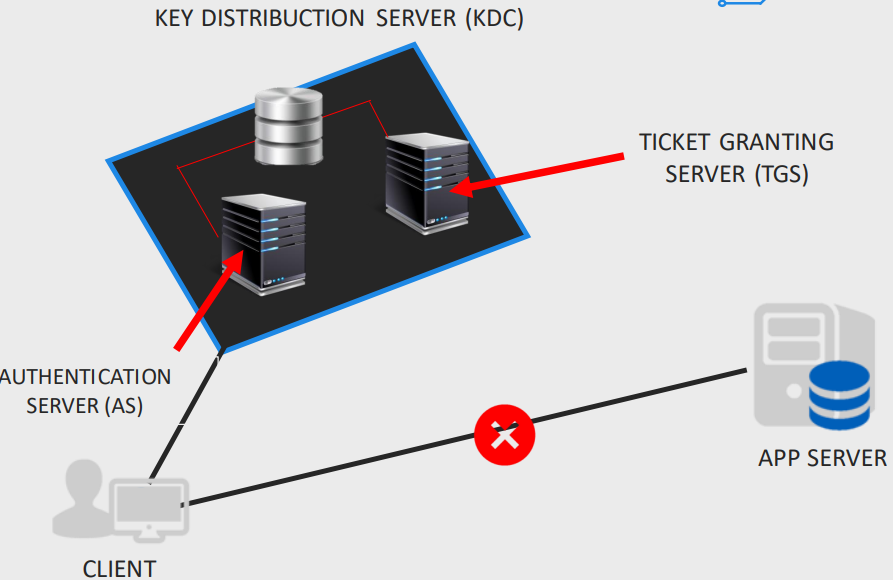
\includegraphics[width=6.26772in,height=3.76389in]{media/image61.png}

Problema della ricerca

In molte applicazioni è necessario ricercare un elemento all'interno di
una struttura dati senza saperne la posizione, o non potendovi accedere
direttamente.

La formulazione del problema della ricerca si basa su:

\begin{itemize}
\item
  \textbf{modalità di accesso} (casuale,sequenziale,...);
\item
  \textbf{rappresentazione della posizione dell'elemento} (es. indice,
  puntatore, ...);
\item
  \textbf{rappresentazione della proprietà dell'elemento} (es. valore,
  predicato sul valore, posizione...);
\end{itemize}

Usando un accesso di tipo \textbf{casuale} l'\emph{\ul{accesso}} ad un
elemento è \emph{\ul{costante}} indipendentemente dall posizione
{[}\(\Theta(1)\){]} invece usando l'accesso \textbf{sequenziale} tutto
\emph{\ul{dipende dalla distanza}} tra l'elemento desiderato e l'ultimo
elemento acceduto (tra \(x_{i}\) e \(x_{j}\) è \(\Theta(|i - j|)\).

Negli esempi successivi si userà un \textbf{array} quindi una struttura
dati con le seguenti proprietà:

\begin{itemize}
\item
  \textbf{modalità d'accesso}: accesso casuale;
\item
  \textbf{rappresentazione posizione}: attraverso indice
\item
  \textbf{rappresentazione proprietà}: mediante una nozione di
  uguaglianza \emph{equal} che deve essere:

  \begin{itemize}
  \item
    \textbf{riflessiva}: \emph{equal(a,a)};
  \item
    \textbf{simmetrica}: \emph{equal(a,b)} \(\Rightarrow\)
    \emph{equal(b,a)\textbf{;}}
  \item
    \textbf{transitica}: \emph{equal(a,b)} \(\land\) \emph{equal(b,c)}
    \(\Rightarrow\) \emph{equal(a,c)}.
  \end{itemize}
\end{itemize}

\textbf{Def \textbar{} Ricerca su sequenza indicizzata}

Data una sequenza indicizzata di elementi \(a_{1}....a_{n}\) e un valore
\(x\) da ricercare, si vuole trovare un indice i tale che
\emph{equal}(\(a_{i},x\)) è vera.

\section{Tipi di ricerca}\label{tipi-di-ricerca}

\subsection{Lineare}\label{lineare}

l'idea è quella di esaminare in sequenza tutti gli elementi della
struttura dati, confrontandoli con l'elemento desiderato:

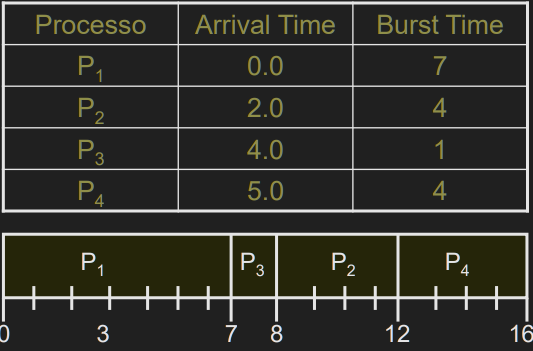
\includegraphics[width=6.26772in,height=1.34722in]{media/image48.png}

Questo algoritmo ha una crescita lineare nel caso medio/peggiore, per
quanto riguarda l'analisi della complessità:

\begin{itemize}
\item
  \textbf{Caso migliore}:
  \(k\  = \ 1:\ T_{best}(n) = \Theta(1) + \Theta(1) = \Theta(1)\)
\item
  \textbf{Caso peggiore}:
  \(k\  = \ n:\ T_{worst}(n) = \Theta(n) + \Theta(1) = \Theta(n)\)
\item
  \textbf{Caso medio}:
  \(k\  = \ n/2:\ T_{avg}(n) = \frac{n}{2}\Theta(1) + \Theta(1) = \Theta(\frac{n}{2}) + \Theta(1) = \Theta(n)\)
\end{itemize}

\subsubsection{Minimo/massimo}\label{minimomassimo}

Adattando l'algoritmo precedente, in quanto la proprietà non è più
verificabile in modo indipendente per ogni elemento, possiamo fare una
ricerca del minimo/massimo in una lista non ordinata di numeri; l'idea
dietro è quella di tenere traccia del risultato parziale.

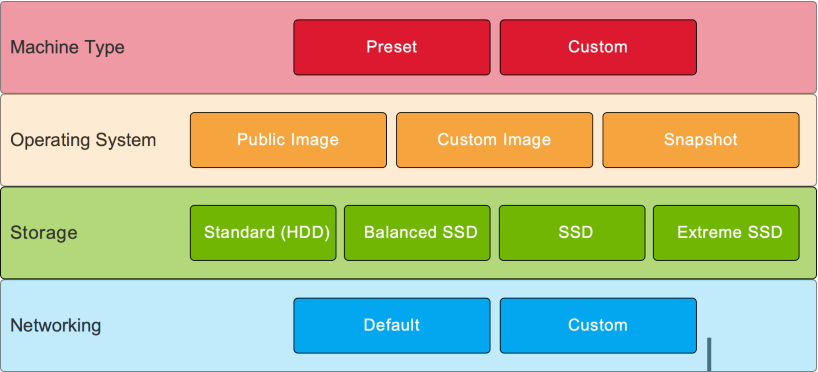
\includegraphics[width=6.26772in,height=1.65278in]{media/image37.png}

\emph{Per qualunque coppia di oggetti x e y dev'essere definita una
relazione Booleana better (x, y) che dice se x dev'essere preferito a y}

\subsection{Binaria}\label{binaria}

in alcuni casi la struttura dati d'ingresso può essere già ordinata,
quindi possiamo assumere che gli elementi dell'array siano ordinati
rispetto a una relazione d'ordine \emph{less}, dove il primo elemento è
minore rispetto al successivo, o \emph{equal} dove due elementi
adiacenti sono uguali.

\emph{Utile per il gioco guess a number o un dizionario}

In questo algoritmo per trovare un numero all'interno della struttura
dati (ordinata) servirà tenere traccia della porzione dell'array da
esaminare usando due indici, \emph{from} e \emph{to}, che tengono
traccia del primo e ultimo elemento utile. In questo modo si andrà a
scartare la porzione di array che non ci interessa.

Ad ogni iterazione scegliamo un elemento utile, detto \textbf{pivot}
(\(x_{m}\)), contenuto fra from e to, verifichiamo se il pivot è
l'elemento da ricercare, se \emph{sì} terminiamo altrimenti restringiamo
il campo:

\begin{itemize}
\item
  \emph{less(elem,} \(x_{m}\)\emph{)}: poniamo to = m − 1;
\item
  \emph{¬less(elem,}\({\ x}_{m}\)\emph{)}: poniamo from = m + 1.
\end{itemize}

Dobbiamo anche considerare che, se l'elemento desiderato non è contenuto
nell'array, la riduzione della porzione da esaminare si ridurrà
all'insieme vuoto.

E per scegliere un elemento utile nella porzione \emph{from..to}
conviene usare la seguente formula: \emph{(from + to)/2 = from/2 +
to/2}.

\emph{Visualizzazione del procedimento}

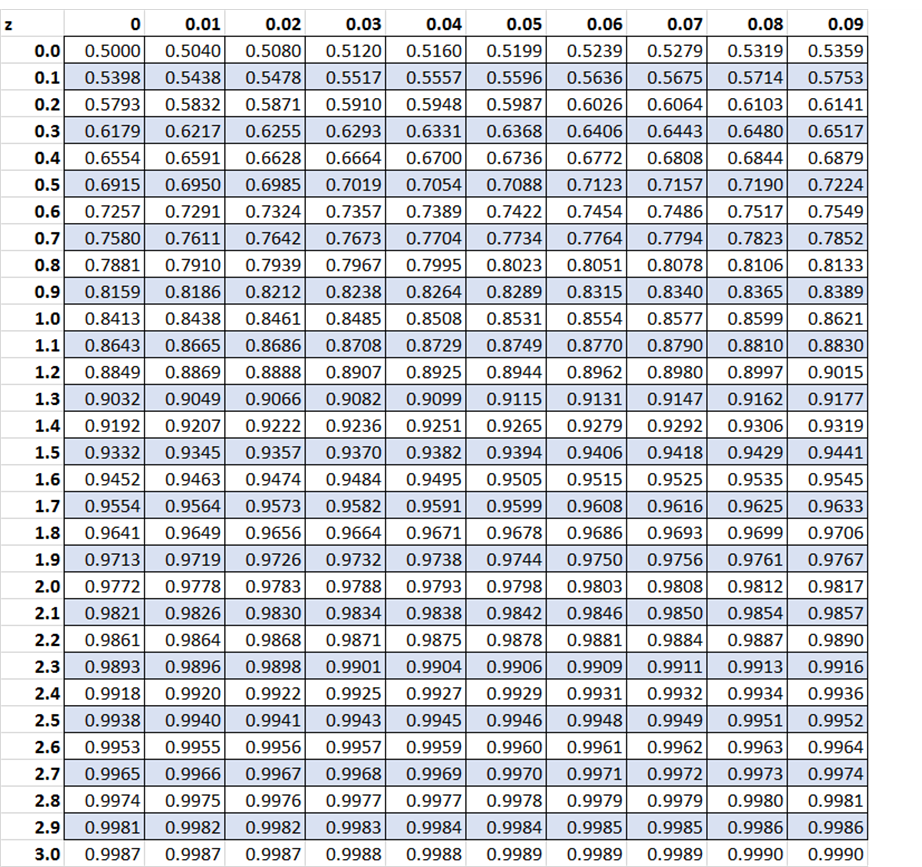
\includegraphics[width=6.26772in,height=3.01389in]{media/image9.png}

L'algoritmo in pseudocodice è il seguente:

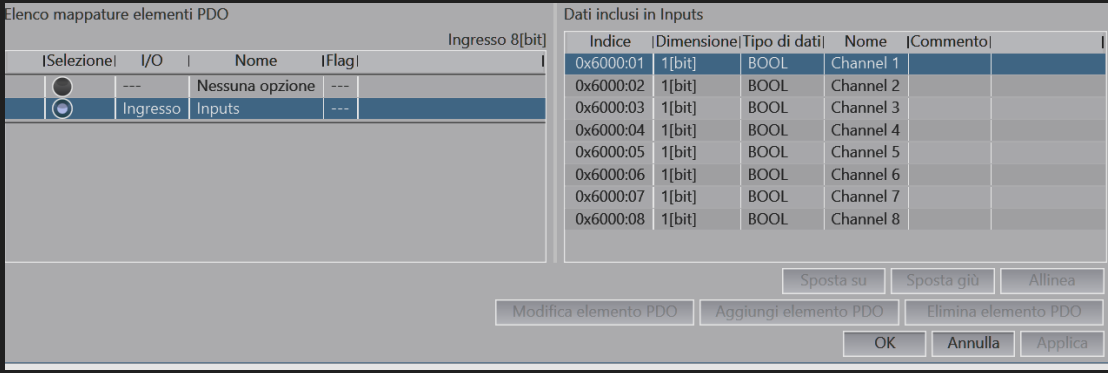
\includegraphics[width=6.26772in,height=2.19444in]{media/image72.png}

L'analisi della complessità denota che nel caso generale
\(T(n) = k\Theta(1)\) e nel migliore \(T_{best}(n) = \Theta(1)\). Il
caso peggiore è quando l'elemento non viene trovato quindi
\(T_{worst} = \log_{2}(n)\Theta(1) = \Theta(\log_{2}(n))\) con una
crescita logaritmica.

\section{Per interpolazione / Interpolation
search}\label{per-interpolazione-interpolation-search}

La ricerca per interpolazione è una variante migliorata della ricerca
binaria, che si basa sull'interpolazione \emph{{[}metodo per individuare
nuovi punti del piano cartesiano a partire da set finito di punti
dati{]}}.

In questo algoritmo, per cercare di indovinare dove sarà l'elemento da
ricercare, si usa la formula:

\(x = x_{0} + \frac{(x_{1} - x_{0}) \cdot ({y - y}_{0})}{y_{1} - y_{0}}\)

Dove:

\begin{itemize}
\item
  Gli indici da considerare sono quelli dell'intervallo {[}\(x_{0}\),
  \(x_{1}\){]}
\item
  La formula offre una ``stima'' di dove è plausibile si possa trovare
  il target da trovare considerando:

  \begin{itemize}
  \item
    \((x_{1} - x_{0})\): la grandezza dell'intervallo considerato;
  \item
    \((y - y_{0})\): la differenza tra il target da trovare e il più
    piccolo esaminato;
  \item
    \((y_{1} - y_{0})\): la differenza tra il più grande e il più
    piccolo nell'intervallo esaminato;
  \end{itemize}
\end{itemize}

\emph{Esempio di esecuzione {[}caso sfortunato{]}}

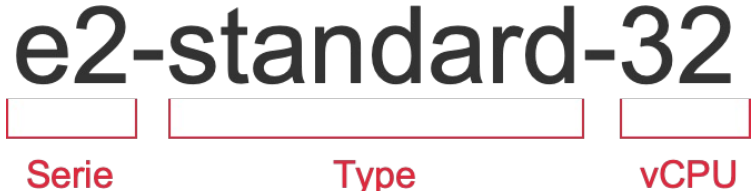
\includegraphics[width=6.01563in,height=3.18171in]{media/image33.png}

L'algoritmo in pseudocodice è il seguente:

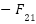
\includegraphics[width=6.26772in,height=2.43056in]{media/image14.png}

Per quanto riguarda l'analisi della complessità:

\begin{itemize}
\item
  \textbf{Caso migliore}: \(O(1)\)
\item
  \textbf{Caso medio}: \(O(log\ log\ n)\)
\item
  \textbf{Caso peggiore}: \(O(n)\)
\end{itemize}

Strutture dati di base

\section{Array dinamici}\label{array-dinamici}

Si superano i problemi degli array classici come l'impossibilità di
modificarlo a run-time o operazioni simili che hanno complessità
\(\Theta(n)\).

L'allocazione in memoria può essere:

\begin{itemize}
\item
  \textbf{Statica}: il ciclo di vita del programma e dell'oggetto è
  uguale (creati/distrutti insieme);
\item
  \textbf{Automatica}: l'oggetto viene de/allocato automaticamente
  all'uscita/entrata di un contesto;
\item
  \textbf{Dinamica}: l'oggetto viene allocato e deallocato su richiesta
  (malloc, free).
\end{itemize}

In maniera simile una \textbf{struttura dati è} \emph{statica} se ha
\ul{dimensione fissa} o \emph{dinamica} se \ul{varia a run time}.

\emph{Recap C:}

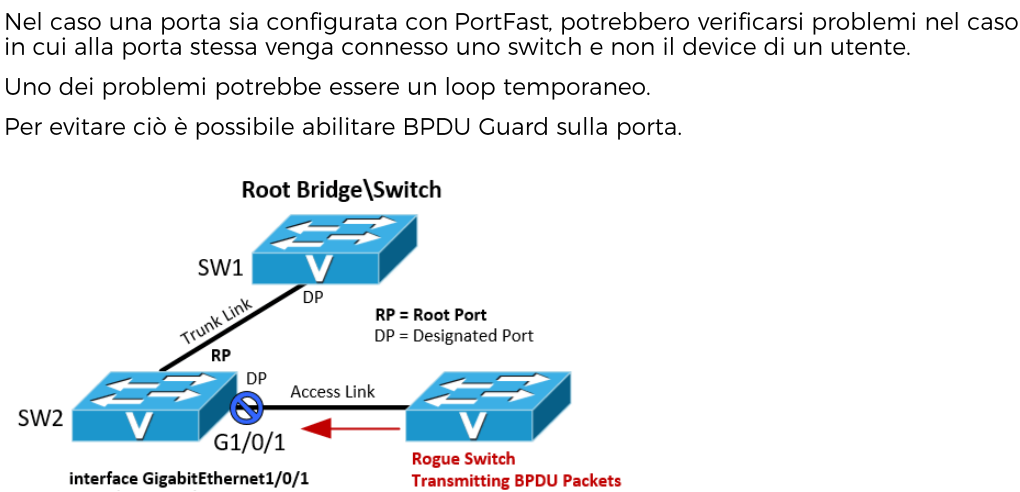
\includegraphics[width=4.79186in,height=2.10938in]{media/image15.png}

In linguaggi nuovi come Python gli array dinamici sono già presenti
sotto forma di liste, in C questo non è vero.

Per realizzarle abbiamo bisogno di funzioni per gestire dinamicamente la
memoria, la cosiddetta \textbf{riallocazione}, e tenere traccia della
dimensione corrente.

La riallocazione è un'operazione costosa (\(\Theta(n)\)) e quindi
evitiamo di farla ogni cambio di dimensione, a questo punto distinguiamo
tra:

\begin{itemize}
\item
  \textbf{Capacità}: numero max di elementi contenuti;
\item
  \textbf{Dimensione/Lunghezza}: numero di elementi correnti all'interno
  della struttura dati.
\end{itemize}

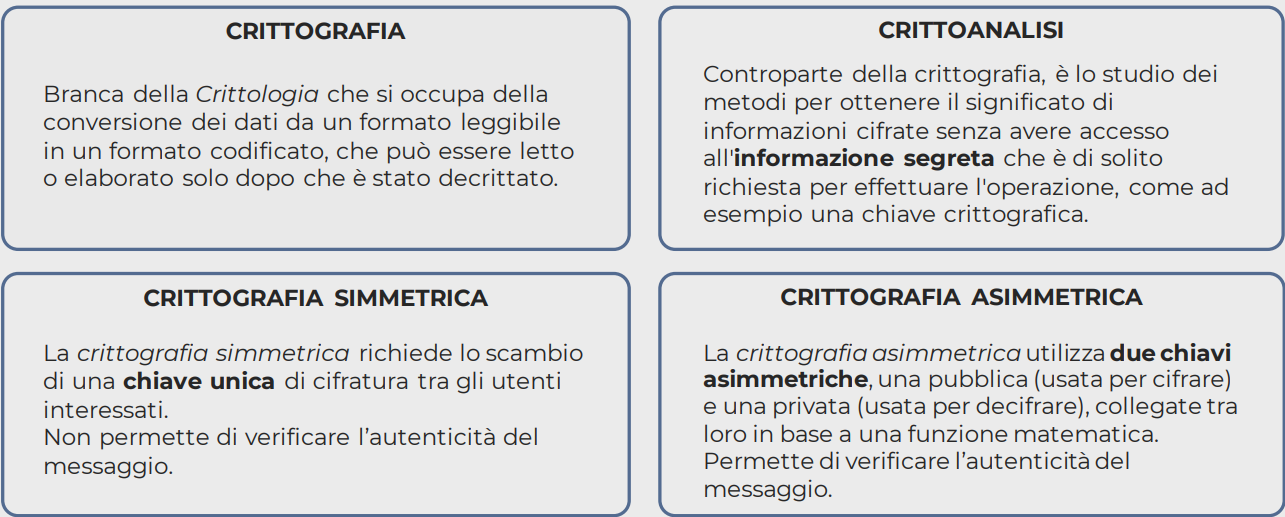
\includegraphics[width=6.26772in,height=1.19444in]{media/image20.png}

Per lavorare sulle due variabili distinguiamo fra:

\begin{itemize}
\item
  \textbf{Ridimensionamento}: lavora sulla size;
\item
  \textbf{Riallocazione}: lavora sulla capacity, operazione che viene
  fatta meno di frequente e solo quando la size è piena.
\end{itemize}

Se abbiamo una \textbf{espansione} vuol dire che:
\(size\  < \ newSize\), ma c'è bisogno di ridimensionare con
riallocazione solo se: \(capacity\  < \ newSize\). Con una
\textbf{contrazione} invece abbiamo che: \(newSize\  < \ size\) e la
riallocazione è necessaria.

Ora però dobbiamo capire quanta capacità supplementare va allocata o
tollerata in queste due fasi.

\subsection{Ridimensionamento con espansione
lineare}\label{ridimensionamento-con-espansione-lineare}

Distinguiamo in riallocazione e contrazione:

\begin{itemize}
\item
  in caso di necessità di \emph{riallocazione}
  (\(capacity\  < \ newSize\)), riserviamo un numero fisso di elementi
  in più \(\Delta_{grow}\) rispetto alla dimensione richiesta:
\end{itemize}

\begin{quote}
\(capacity\  < \ newSize \Rightarrow newCapacity \leftarrow newSize + \Delta_{grow}\)
\end{quote}

\begin{itemize}
\item
  in caso di contrazione, riduciamo la capacità solo se la differenza
  tra la capacità attuale e la nuova lunghezza richiesta supera una
  soglia \(\Delta_{shrink}\):
\end{itemize}

\begin{quote}
\(capacity - newSize > \Delta_{shrink} \Rightarrow newCapacity \leftarrow newSize + \Delta_{grow}\)

\emph{Ricordarsi di controllare che}
\(\Delta_{grow} \leq\)\(\Delta_{shrink}\)
\end{quote}

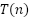
\includegraphics[width=6.26772in,height=1.36111in]{media/image5.png}

\subsection{Ridimensionamento con espansione
geometrica}\label{ridimensionamento-con-espansione-geometrica}

In questo caso invece di usare una capacità supplementare fissa
\(\Delta_{grow}\) si usa una capacità supplementare che è proporzionale
alla lunghezza richiesta \(newSize\) di un fattore \(\phi_{grow} > 1\).

In caso di contrazione riduciamo la capacità quando:
\((capacity/newSize) > \phi_{shrink} > 1\), quindi i possibili frangenti
sono:

\begin{enumerate}
\def\labelenumi{\arabic{enumi}.}
\item
  Se \(capacity\  < \ newsize\) allora
  \(newCapacity \leftarrow \phi_{grow} \cdot newSize\)
\item
  Se \((capacity/newSize) > \phi_{shrink}\) e con
  \(\phi_{shrink} \geq \phi_{grow}\ \) allora
  \(newCapacity \leftarrow \phi_{grow} \cdot newSize\)
\item
  nessuna riallocazione
\end{enumerate}

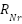
\includegraphics[width=6.26772in,height=1.22222in]{media/image53.png}

\subsection{Complessità}\label{complessituxe0}

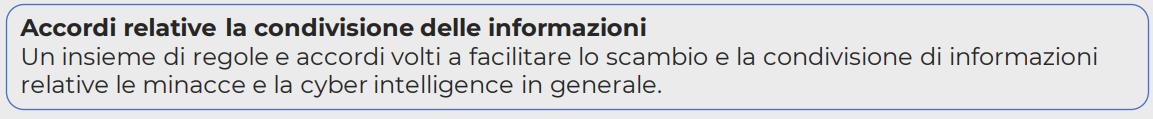
\includegraphics[width=4.95313in,height=1.64556in]{media/image88.png}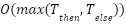
\includegraphics[width=4.97493in,height=2.85108in]{media/image50.png}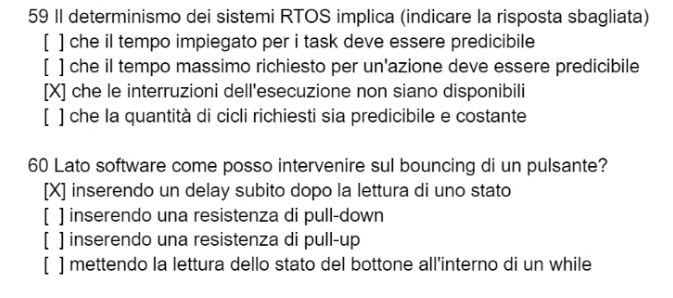
\includegraphics[width=4.97087in,height=2.86527in]{media/image21.png}

\section{Pile / Stack}\label{pile-stack}

Struttura dati con accesso di tipo LIFO, l'ultimo elemento che entra è
il primo ad uscire. Le operazioni possibili sono:

\begin{itemize}
\item
  \emph{create} e \emph{destroy};
\item
  \emph{push}: metti in cima;
\item
  \emph{pop}: togli dalla cima;
\item
  \emph{top}: vedi cosa c'è in cima;
\item
  \emph{isempty} e \emph{isfull}: controllo vuota/piena.
\end{itemize}

Per implementare una pila è sufficiente tenere traccia del numero di
elementi presenti e da questo dato si ricava anche la posizione di
inserimento o prelievo. L'implementazione risulta facile tramite array
(statico o dinamico):

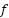
\includegraphics[width=3.7843in,height=2.04302in]{media/image44.png}

Dove \emph{n} tiene traccia del numero di elementi e allo stesso tempo
della prossima posizione di inserimento

\section{Code / Queue}\label{code-queue}

Struttura dati con modalità di accesso FIFO, il primo elemento che entra
è il primo ad uscire.

Utile se vogliamo processare una sequenza di richieste in base
all\textquotesingle ordine di arrivo e con un'attesa non infinita,
possiamo usare i \textbf{buffer} se o il tasso di arrivo di richieste
(producer speed) non corrisponde alla capacità di soddisfarle (consumer
speed)o il tasso di arrivo di richieste (producer speed) non corrisponde
alla capacità di soddisfarle (consumer speed).

Le operazioni possibili sono:

\begin{itemize}
\item
  \emph{create} e \emph{destroy};
\item
  \emph{add} o \emph{enqueue}: metti in coda o accodamento;
\item
  \emph{remove} o \emph{dequeue}: togli dalla coda;
\item
  \emph{front}: vedi cosa c'è in cima (1° elemento);
\item
  \emph{isempty} e \emph{isfull}: controllo vuota/piena.
\end{itemize}

Per implementare una coda è sufficiente tenere traccia del numero di
elementi presenti e da questo dato si ricava anche la posizione di
inserimento o prelievo.

Tenendo traccia della testa (\(f\)), il prelievo si attua semplicemente
con lo spostamento in avanti di \(f\).

Si può sempre usare un array statico o dinamico e \emph{per evitare
problemi di complessità} la soluzione è implementare una \textbf{coda
circolare} dove \emph{l'array viene interpretato come struttura ciclica}
(dove la posizione successiva all'ultima è quella di indice 0) e per
incrementare gli indici è comodo usare la capacity:

Enqueue: \(b = (b + 1)\% capacity\) \textbar{} Dequeue:
\(f = (f + 1)\% capacity\)

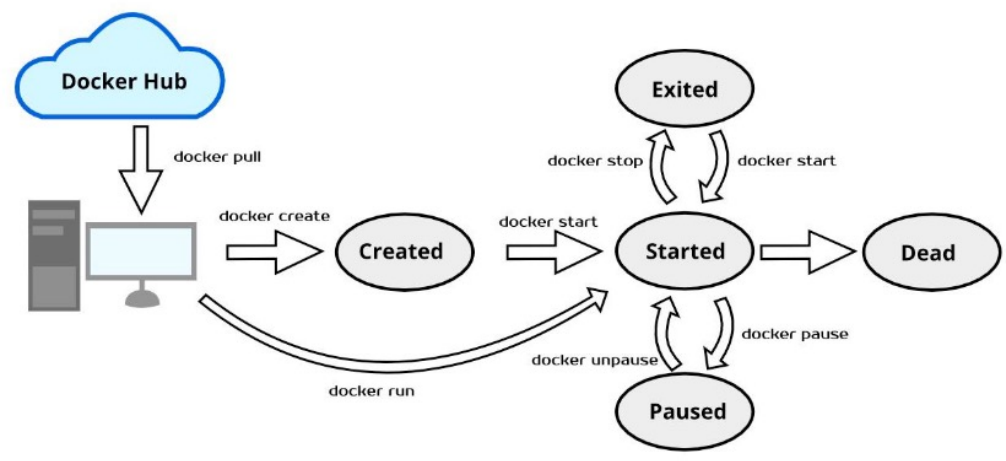
\includegraphics[width=3.77604in,height=0.94715in]{media/image66.png}

Liste dinamiche

Utili per rappresentare collezioni di elementi organizzati linearmente e
per lavorare con collezioni che consentano di svolgere in modo
efficiente le operazioni di ricerca, inserimento, e cancellazione.

\textbf{Def \textbar{} Lista}: \emph{struttura dati che immagazzina un
insieme di elementi in ordine}

Esistono diversi tipi di liste:

\begin{itemize}
\item
  \textbf{Linked list}: formata da nodi, ogni nodo contiene
  l'informazione e il riferimento all'elemento successivo.
\end{itemize}

\begin{quote}
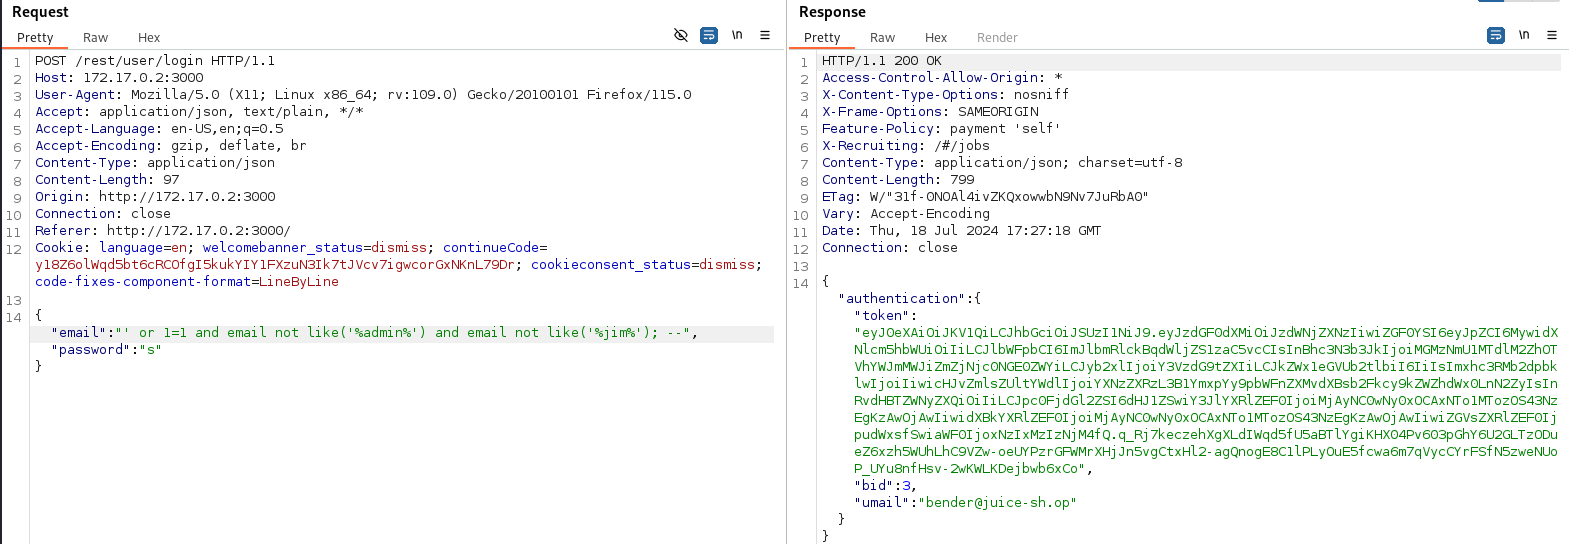
\includegraphics[width=4.52604in,height=0.4511in]{media/image16.png}

L'ordine degli elementi è dato dai collegamenti esistenti fra gli
elementi e non dal piazzamento in memoria, il primo elemento è la
\emph{testa} e l'ultimo è la \emph{coda}.
\end{quote}

\begin{itemize}
\item
  \textbf{Doubly-linked list}: ogni nodo contiene anche un collegamento
  all'elemento precedente; tipicamente sono noti sia il riferimento alla
  testa sia il riferimento alla coda.
\end{itemize}

\begin{quote}
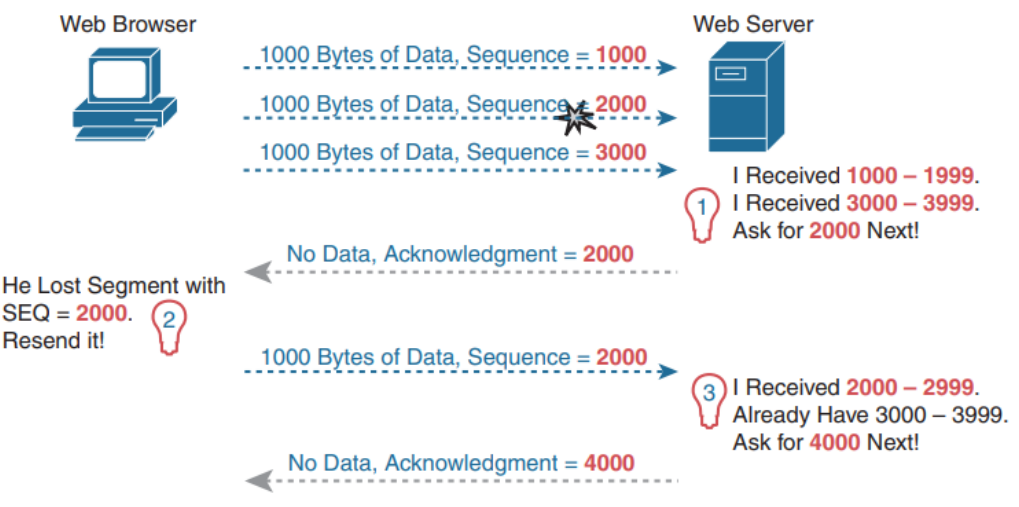
\includegraphics[width=4.59531in,height=0.72065in]{media/image75.png}
\end{quote}

\begin{itemize}
\item
  \textbf{Circular list}: una linked list dove l'elemento in coda è
  collegato all'elemento in testa, il collegamento può essere singolo o
  doppio.
\end{itemize}

\begin{quote}
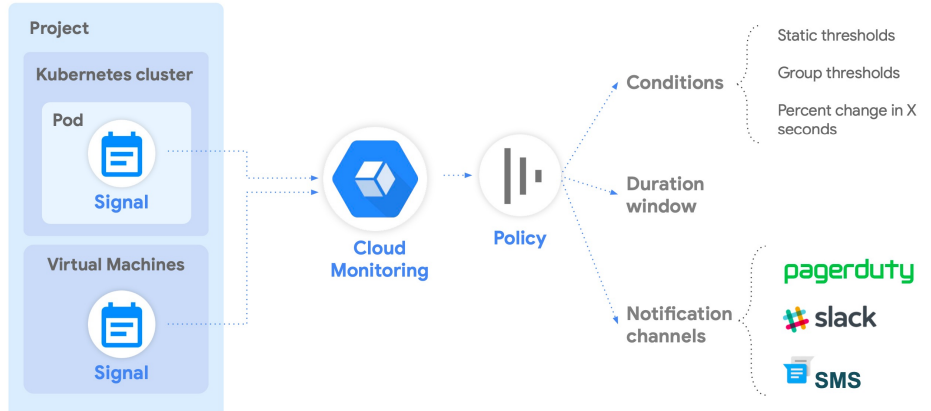
\includegraphics[width=4.41218in,height=0.93814in]{media/image28.png}
\end{quote}

Possiamo distinguere tre nozioni di ordinamento nelle liste:

\begin{enumerate}
\def\labelenumi{\arabic{enumi}.}
\item
  \emph{Ordine strutturale:} l'ordine risultante dai collegamenti fra i
  nodi;
\item
  \emph{Ordine logico:} l'ordine esistente tra gli elementi sulla base
  di una relazione d'ordine;
\item
  \emph{Ordine fisico}: l'ordine degli elementi in memoria.
\end{enumerate}

\textbf{Def \textbar{} Lista ordinata}: \emph{una lista dove l'ordine
strutturale corrisponde all'ordine logico}

\section{Implementazione}\label{implementazione}

L'implementazione può avvenire su array statici o dinamici dove ogni
elemento dell'array è un nodo della lista e il collegamento è dato
dall'indice dell'elemento successivo. Con gli array statici c'è il
problema di quanta memoria allocare e nei dinamici della rimozione dei
nodi e della frammentazione della memoria contigua associata all'array
dinamico.

Normalmente l'implementazione avviene tramite allocazione dinamica dei
nodi, si definisce la lista come struttura dati ricorsivamente definita:

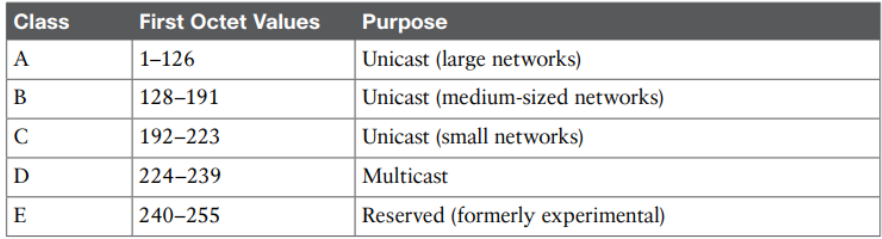
\includegraphics[width=6.26772in,height=0.70833in]{media/image84.png}

Una \emph{list} può essere \textbf{NULL}, se è vuota, oppure un nodo che
contiene un \textbf{value} e il collegamento \textbf{next} alla
sottolista rimanente:

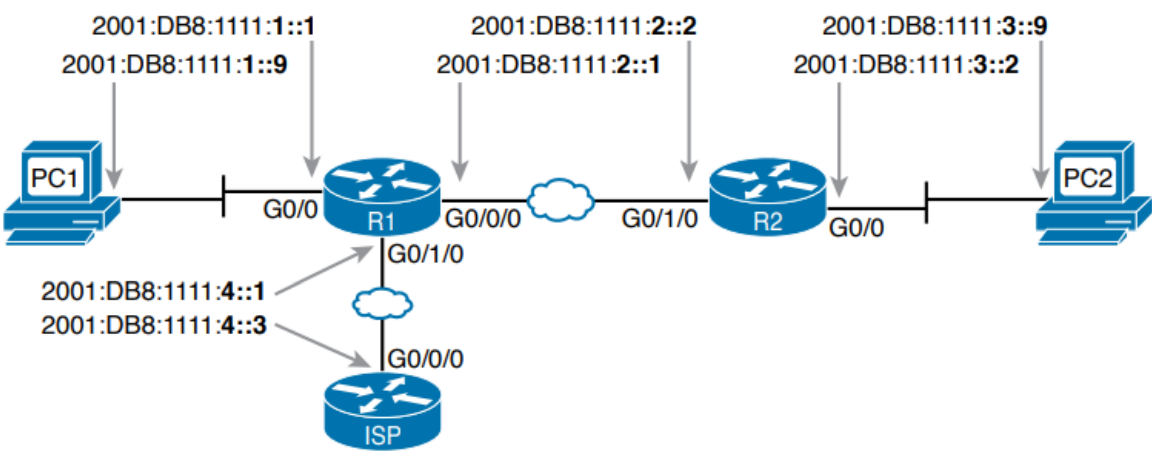
\includegraphics[width=6.26772in,height=0.94444in]{media/image68.png}

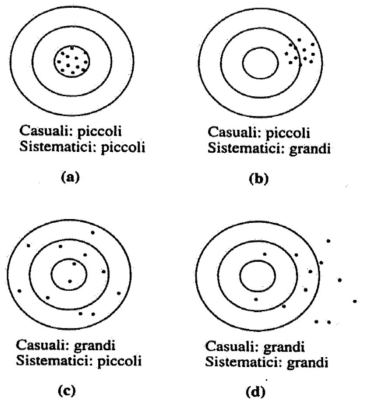
\includegraphics[width=6.43311in,height=3.58207in]{media/image80.png}

Ora vediamo una carrellata di operazioni utili per lavorare con le
liste:

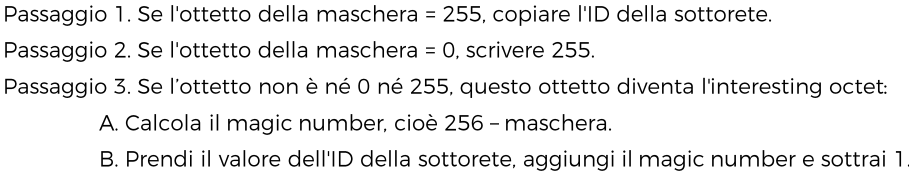
\includegraphics[width=5.99688in,height=2.87276in]{media/image73.png}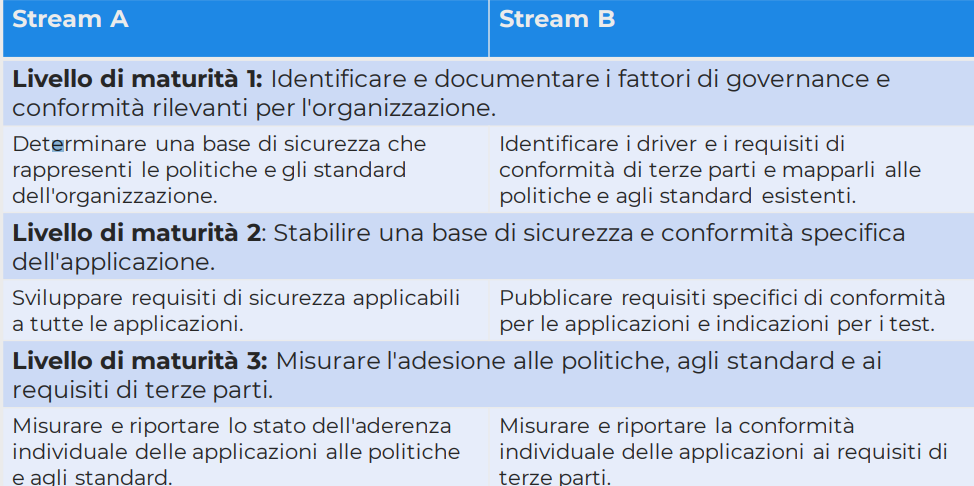
\includegraphics[width=5.94427in,height=2.91944in]{media/image87.png}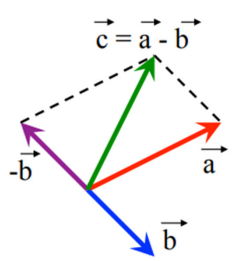
\includegraphics[width=5.7763in,height=2.53646in]{media/image67.png}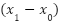
\includegraphics[width=5.9026in,height=1.65192in]{media/image86.png}

L\textquotesingle inserimento ha complessità \(\Theta(1)\) nel caso
migliore e \(\Theta(n)\) nel peggiore/medio. Le stesse complessità
valgono per rimozione e ricerca.

\section{Liste vs Array dinamici}\label{liste-vs-array-dinamici}

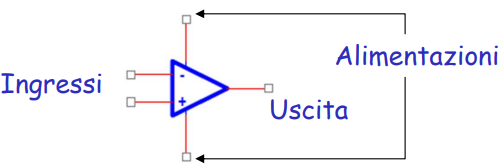
\includegraphics[width=6.26772in,height=1.80556in]{media/image81.png}

Tabelle hash

Create per supportare ricerche con complessità \(\Theta(1)\), ecco la
definizione:

\emph{Una tabella (anche chiamata mappa o dizionario o array
associativo) è un insieme di coppie chiave-valore (elementi)}
\(E_{i} = (K_{i},V_{i})\)\emph{. Le chiavi sono prese da un insieme}
\(U\) \emph{(universo delle chiavi), gli elementi da un insieme V.}

In questo caso la chiave identifica un certo elemento, ma esistono
strutture dati dove ad ogni chiave può corrispondere più di un elemento,
la \textbf{multi-mappa}.

Operazioni possibili:

\begin{itemize}
\item
  \emph{insert(key, elem)}: inserimento della coppia (k,e) alla mappa;
\item
  \emph{get(k)}: restituzione dell'elemento associato alla chiave k;
\item
  \emph{delete(k)}: rimozione elemento associato alla chiave.
\end{itemize}

\section{A indirizzamento diretto}\label{a-indirizzamento-diretto}

\emph{Si fa uso di} un \textbf{vettore} e usa \textbf{chiavi numeriche}
il cui valore è da interpretarsi come indice del vettore.

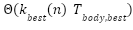
\includegraphics[width=5.36979in,height=1.68587in]{media/image59.png}

\emph{Fattore di carico}: \(n = n/m\) per \(n\) chiavi/elementi
memorizzati, un esempio:

Se usiamo un codice da 4 cifre possiamo usare un array di 10000 elementi
e usare il codice come chiave.

Avendo 500 elementi, il fattore di carico è:
\(n = 500/10000 = 0.05 = 5\%\)

\section{A indirizzamento indiretto}\label{a-indirizzamento-indiretto}

Riduce l'occupazione di memoria avendo comunque un accesso efficiente.
la strategia è usare la funzione di hash
\(h:U \rightarrow \lbrack 0,1,...,m - 1\rbrack\) che fa corrispondere ad
ogni chiave \emph{k} appartenente a \emph{U} la posizione nell'array in
cui l'informazione associata è memorizzata.

\emph{La dimensione m può non coincidere con} \(|U|.\)

Quando due chiavi (\(k_{1}e{\ k}_{2}\)) hanno lo stesso valore hash
(\(h(k_{1}) = h(k_{2})\)) si verifica una \textbf{collisione}.

Se una funzione (\emph{h}) non causa collisioni, cioè è iniettiva, si
chiama \textbf{hash perfetto}.

\(\forall k_{1},k_{2} \in U,\ k_{1} \neq k_{2} \Rightarrow h(k_{1}) \neq h(k_{2})\)

Si dice \textbf{hash perfetto minimale} un hash (\emph{h}) con immagine
da 0 a \((|U| - 1)\).

Per la gestione delle collisioni esistono due metodi:

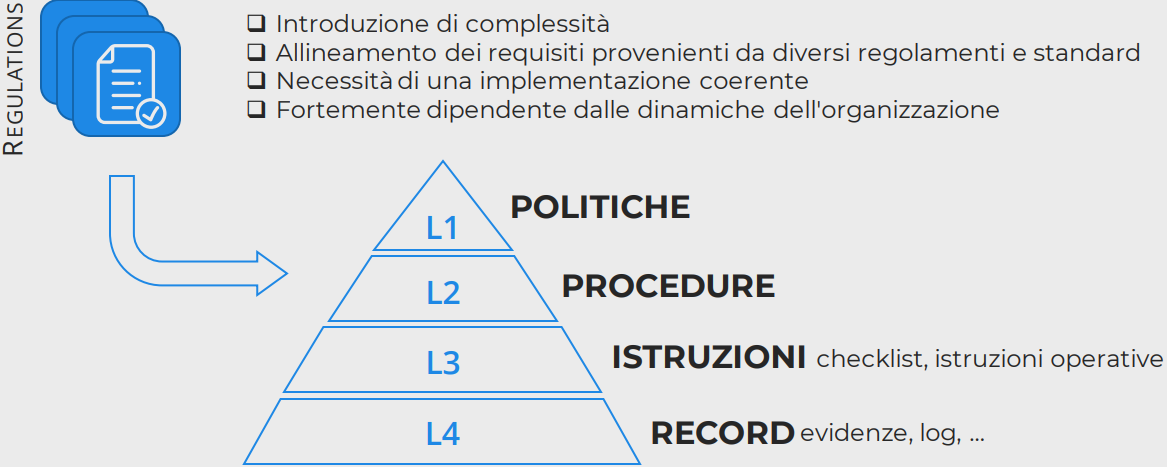
\includegraphics[width=6.26772in,height=3.31944in]{media/image18.png}

Una buona funzione di hash deve essere facile da calcolare e distribuire
in modo uniforme le chiavi sulle posizioni della tabella.

Con la distribuzione uniforme le liste di collisione devono avere
lunghezza \(n/m = 2\), con complessità di accesso worst-case:
\(\Theta(n/m)\); senza si avrebbe \(\Theta(l_{\max})\) con \(l_{\max}\)
= lunghezza della lista di collisione più lunga.

Ogni chiave, secondo l'\textbf{uniformità semplice,} deve avere la
stessa probabilità di vedersi assegnata una qualsiasi posizione
ammissibile indipendentemente da altri valori hash già assegnati; il
requisito di uniformità semplice è difficile da verificare.

\subsection{Funzioni di hash}\label{funzioni-di-hash}

Il \textbf{metodo della divisione} è semplice e veloce, la formula è la
seguente:

\(h(k) = k \cdot mod \cdot m\)

Conviene evitare certi valori di \emph{m}, come le potenze di 2, occorre
rendere \emph{h} dipendente da tutti i bit della chiave per questo
\emph{m} dovrebbe essere un numero primo non troppo vicino ad una
potenza del due.

Il \textbf{metodo della moltiplicazione} ha la seguente formula:

\(h(k) = \lfloor m \cdot (k \cdot A - \lfloor k \cdot A\rfloor)\rfloor\)

Per sapere cosa vuol dire il simbolo:
\href{https://it.wikipedia.org/wiki/Parte_intera}{⌊}

Consiste in due passi:

\begin{enumerate}
\def\labelenumi{\arabic{enumi}.}
\item
  si moltiplica la chiave \(k\) per una certa costante \(A\),
  \(0 < A < 1\), estraendo la parte frazionaria \(k \cdot A\);
\item
  moltiplico la parte frazionaria per \(m\) e prendo la parte intera
  inferiore del risultato.
\end{enumerate}

\(k \cdot A -\)\(\lfloor k \cdot A\rfloor\) è la parte frazionaria di
\(k \cdot A\) (si suggerisce: \(A \approx ( - 1)/2\))

In questo metodo \emph{m} non è critico.

\section{Implementazione hashtable}\label{implementazione-hashtable}

\subsection{Chained hashtable}\label{chained-hashtable}

Una \textbf{chained hashtable} (aka separate chaining o closed
addressing hash table) è una impl. di tabelle ad indirizzamento
indiretto che usa liste di collisione.

Per implementarli si usa un vettore di bucket, dove ogni bucket vi è una
linked list:

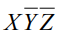
\includegraphics[width=6.26772in,height=2.84722in]{media/image52.png}

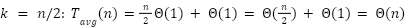
\includegraphics[width=6.26772in,height=3.34722in]{media/image77.png}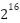
\includegraphics[width=6.26772in,height=1.41667in]{media/image3.png}

Per quanto riguarda la complessità tutte le operazioni sono
\(\Theta(1)\) tranne la \emph{list\_search} con complessità \(O(k)\)
(\emph{k} sta per la lunghezza della lista di collisione).

Se la funzione di hash produce una distribuzione uniforme delle chiave,
si avrà una lunghezza media della lista \(n/m\) e avramo
\(\Theta_{avg}(n) = \Theta(n/m)\) (\emph{n}: numero elementi in tabella,
\emph{m}: numero bucket).

Con un numero di bucket proporzionale al massimo numero di elementi
previsti:
\(\Theta_{avg}(n) = \Theta(n/m) = \Theta(n/(cn)) = \Theta(c) = \Theta(1)\).

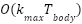
\includegraphics[width=6.26772in,height=2.25in]{media/image62.png}

Anche qui abbiamo \(\Theta_{avg}(n/m)\) e \(\Theta_{worst}(n)\) della
ricerca.

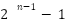
\includegraphics[width=6.26772in,height=1.97222in]{media/image10.png}

La complessità per \(T_{avg} = T_{worst} = \Theta(n)\), ma se
\(m \gg n\) allora avremo; \(T_{worst} = \Theta(m + n)\)

Ora vediamo diverse funzioni di hash per diversi tipi:

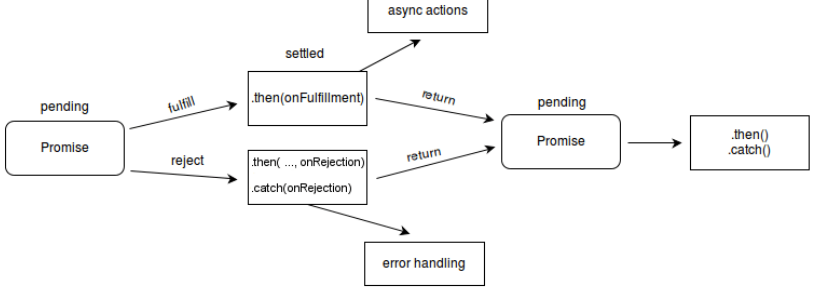
\includegraphics[width=6.26772in,height=0.54167in]{media/image7.png}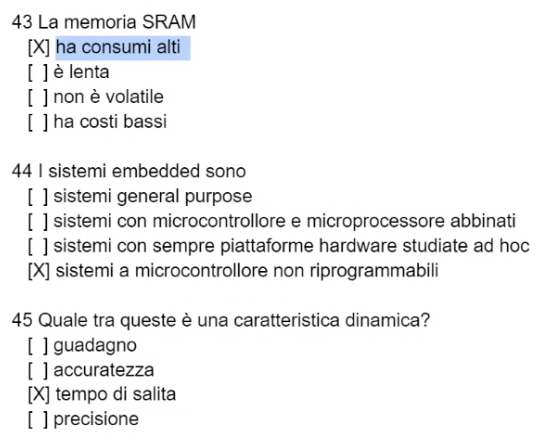
\includegraphics[width=6.26772in,height=1.51389in]{media/image8.png}

Per tipi arbitrari conviene interpretare la struttura dati come sequenza
di byte, e di applicare un algoritmo simile a quello mostrato per le
stringhe; \textbf{però} per valori concettualmente equivalenti occorre
produrre lo stesso hashcode e si interpreti tutto il contenuto della
struttura dati: se questa usa puntatori, si consideri il contenuto
dell'area puntata (e non il puntatore).

\subsection{\texorpdfstring{Probing }{Probing }}\label{probing}

Una \textbf{probing / open addressing hashtable} è una implementazione
di tabelle ad indirizzamento indiretto che memorizza le coppie
chiave-valore direttamente nei bucket dell'array sottostante e usa la
tecnica dell' ispezione/probing lineare per risolvere le collisioni.

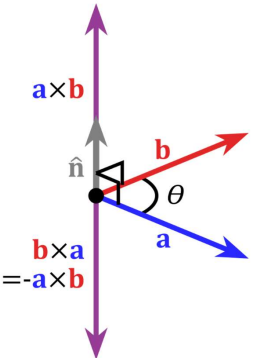
\includegraphics[width=6.26772in,height=2.09722in]{media/image76.png}

Quando \(n \approx m\) il probing causa collisioni aggiuntive e si
raccomanda che il fattore di carico sia sotto una soglia di carico
\(\lambda:n/m < \lambda < 1\), se si supera \(\lambda\) la tabella va
ridimensionata e ricalcolare l'hash di tutti gli elementi
(\emph{re-hasing}).

\section{Set}\label{set}

È una struttura dati che memorizza una collezione di elementi distinti;
quindi senza duplicati e senza un ordine particolare.

Sono mutabili e ogni elemento del set deve essere hashable.

{[}RECAP{]}

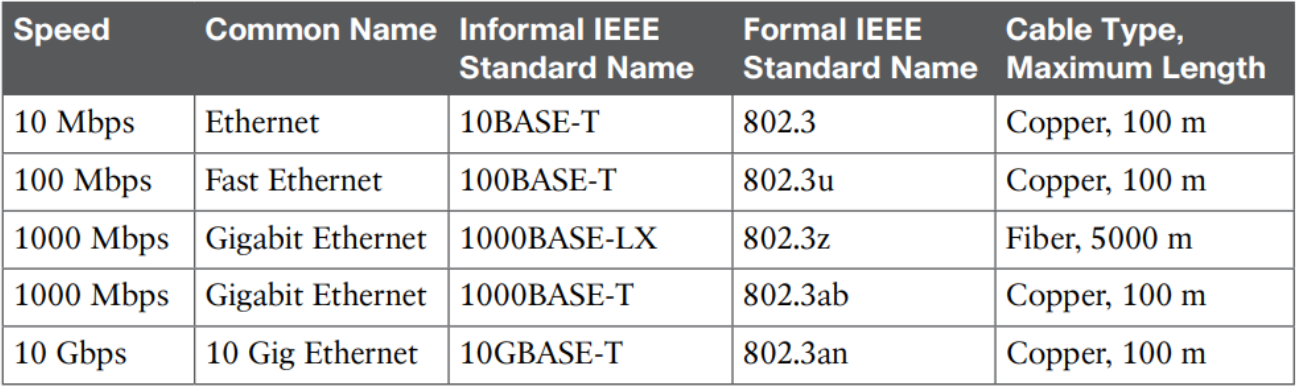
\includegraphics[width=6.26772in,height=3.22222in]{media/image42.png}

Algoritmi di ordinamento

\textbf{Def \textbar{} Sorting:} \emph{Data una sequenza}
\(x_{1},x_{2},....,x_{n}\)\emph{, l'ordinamento di tale sequenza
consiste nel determinare una sua permutazione}
\(x_{1}^{'},x_{2}^{'},\ ....\ ,x_{n}^{'}\) \emph{tale che}
\(x_{1}^{'} \leq x_{2}^{'} \leq \ ....\  \leq x_{n}^{'}\)

L'ordinamento può essere \textbf{interno}, la struttura è interamente
contenuta in memoria centrale, \textbf{esterno}, la struttura è
memorizzata in memoria secondaria.

Un'ulteriore suddivisione è:

\begin{itemize}
\item
  \textbf{ord. sul posto}: detto anche \emph{in-place}, l'output
  consiste in una modifica della struttura in input(complessità spaziale
  di strutture dati aggiuntive al \(max\ O(log(n))\));
\item
  \textbf{ord. fuori posto:} detto anche \emph{out-of-place}, si produce
  una nuova struttura in output (complessità spaziale strutture dati
  aggiuntive \(\Omega(n)\)).
\end{itemize}

L'\textbf{ordinamento stabile} è : quando nella sequenza finale gli
elementi equivalenti mantengono lo stesso ordine relativo.

L'\textbf{ordinamento per confronti}: l'ordinamento è basato sul
confronto di coppie di elementi.

\section{Selection sort}\label{selection-sort}

Si cerca il minimo nell'array da ordinare, e si scambia con quello alla
prima posizione; si seleziona il minimo nell'array restante, e si
scambia con quello alla seconda posizione; e così via.

Bastano \(n - 1\) iterazioni, l\textquotesingle ultimo sarà ordinato per
forza, vediamo un esempio:

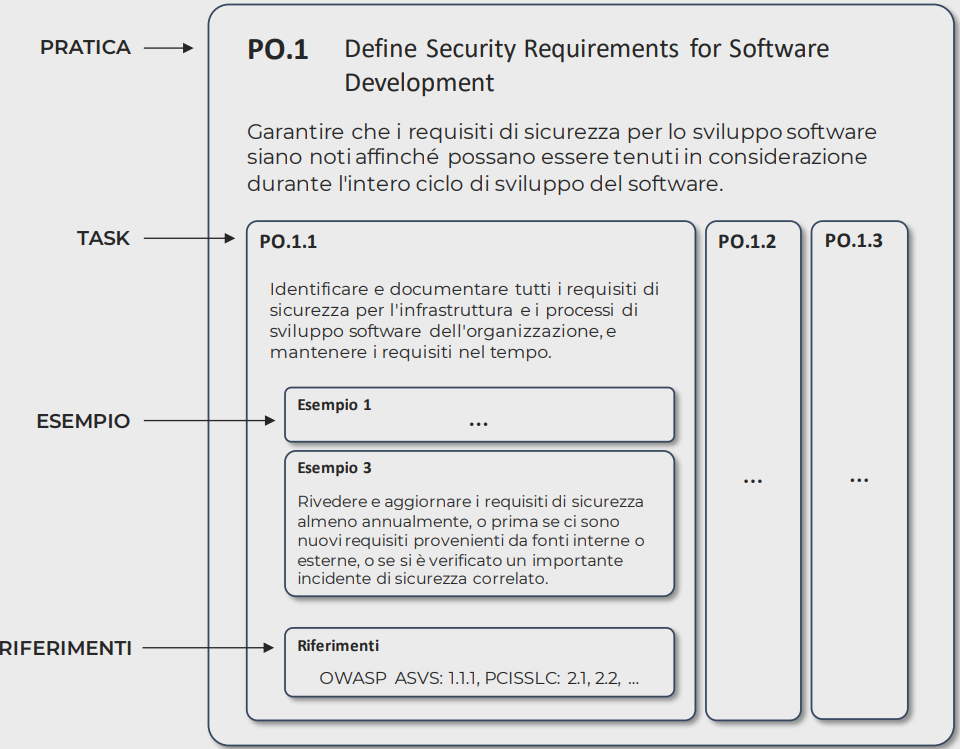
\includegraphics[width=6.26772in,height=1.58333in]{media/image79.png}

In pseudo codice:

\includegraphics[width=6.26772in,height=0.80556in]{media/image34.png}

La complessità è \(\Theta(n^{2})\), ma vediamo perchè:

\(T(n) = \sum_{i = 0}^{n - 2}T^{i}(n)\)

dove \(T^{i}(n)\) è la complessità di una singola iterazione in funzione
della var. i del ciclo

ed essendo che \emph{minIndex} è \(\Theta(n)\) e all'iterazione \emph{i}
lavora su \(n - i\) elementi abbiamo:

\(T(n) = \sum_{i = 0}^{n - 2}\Theta(n - i) = \Theta(\sum_{i = 0}^{n - 2}\Theta(n - i)) = \Theta(\frac{(n - 1)(n + 2)}{2}) = \Theta(n^{2})\)

Alcune osservazioni sul seguente algoritmo possono essere:

\begin{itemize}
\item
  Essendo che lo swap può invertire l'ordine relativo di elem. uguali,
  \textbf{non è stabile!};
\item
  La complessità calcolata precedentemente vale anche per il caso
  migliore.
\end{itemize}

\section{Insertion sort}\label{insertion-sort}

Data una sequenza \(a_{0}....,a_{n - 1}\) già ordinata e un nuovo valore
\(x\), si vuole ottenere una nuova sequenza ordinata di \(n + 1\)
elementi che contenga gli elementi iniziali e \(x\).

Per semplicità dividiamo il problema in due parti

\(\Downarrow\)

\begin{enumerate}
\def\labelenumi{\arabic{enumi}.}
\item
  \emph{Si inizia riducendo il problema
  all\textquotesingle{}\textbf{inserimento in ordine}:}
\end{enumerate}

\begin{quote}
Lo scopo è trovare la posizione dove mettere \emph{x}, per farlo
troviamo la posizione dove si trova il primo elemento più grande, poi
spostiamo tutti i numeri da quella posizione a destra di uno e inseriamo
il nuovo valore nel posto che si è liberato.
\end{quote}

\includegraphics[width=5.38539in,height=1.49395in]{media/image78.png}

\begin{enumerate}
\def\labelenumi{\arabic{enumi}.}
\setcounter{enumi}{1}
\item
  \emph{L'algoritmo in se invece lavora nel seguente modo:}
\end{enumerate}

\begin{quote}
Si tiene traccia di due porzioni dell'array:
\end{quote}

\begin{enumerate}
\def\labelenumi{\arabic{enumi}.}
\item
  la parte iniziale, che è già ordinata;
\item
  la parte finale, da ordinare.
\end{enumerate}

\begin{quote}
Si fa un ciclo che itera sulla seconda parte ed ogni volta prende il
prossimo elemento della parte non ordinata e tramite
\emph{l\textbf{'inserimento in ordine}} lo mette nella parte ordinata
nel posto giusto.
\end{quote}

\includegraphics[width=6.26772in,height=0.30556in]{media/image56.png}\includegraphics[width=6.26772in,height=2.01389in]{media/image71.png}

Un'altra implementazione utilizza due indici: uno punta
all\textquotesingle elemento da ordinare e l\textquotesingle altro
all\textquotesingle elemento immediatamente precedente. Se
l\textquotesingle elemento puntato dal secondo indice è maggiore di
quello a cui punta il primo indice, i due elementi vengono scambiati di
posto; altrimenti il primo indice avanza. Il procedimento è ripetuto
finché si trova nel punto in cui il valore del primo indice deve essere
inserito. Il \emph{primo indice punta inizialmente al secondo}
\emph{elemento dell\textquotesingle array, il secondo inizia dal primo}.
L\textquotesingle algoritmo così tende a spostare man mano gli elementi
maggiori verso destra.

\includegraphics[width=2.50156in,height=1.31481in]{media/image2.png}

L'implementazione, dentro il \emph{while}, sposta a destra di uno il
valore che è in posizione \emph{j} (maggiore dell'elemento da swappare)
e poi diminuisce \emph{j}, in questo modo sposta tutti fino a che non
abbiamo un posto libero per la variabile da swappare (il ciclo si
interrompe o se arriviamo in fondo o finchè non siamo arrivato in un
punto dove il valore di sinistra non è maggiore).

Prima dello swap ci sarà un elemento ripetuto poi in quella posizione
mettiamo l'elemento minore.

La complessità varia nei due algoritmi:

\begin{itemize}
\item
  \emph{insert-in-order}: con \emph{p} la posizione di inserimento

  \begin{itemize}
  \item
    \(T_{iio} = T_{while} + T_{for} = (n - p)\Theta(1) + (n - p)\Theta(1) = \Theta(n - p)\)
  \item
    \textbf{Best case} \emph{{[}}\(p = n\)\emph{{]}}: \(\Theta(1)\);
  \item
    \textbf{Worst case}\emph{{[}}\(p = 0\)\emph{{]}}:\(\Theta(n)\).
  \end{itemize}
\item
  \emph{insertion-sort}:

  \begin{itemize}
  \item
    \(T_{is} = (n - 1)T_{iio}\)
  \item
    \textbf{Best case}: \(\Theta(n)\);
  \item
    \textbf{Worst case}: \(\Theta(n^{2})\).
  \end{itemize}
\end{itemize}

\section{Bubble sort}\label{bubble-sort}

L'idea è di spostare verso la fine dell'array gli elementi che hanno
valore più alto di quelli adiacenti, si esaminano tutte le coppie
adiacenti e se non sono localmente ordinati si scambiano di posto, lo
scambio va registrato e si interrompe il ciclo solo quando non si
registrano più scambi.

Si produrrà un array ordinato in al massimo \(n - 1\) scansioni e per
produrre un ordinamento stabile basta non scambiare i valori adiacenti
con ugual valore.

Visualizzazione del procedimento:

\includegraphics[width=6.26772in,height=2.83333in]{media/image39.png}

Traducendolo in pseudo codice otteniamo:

\includegraphics[width=6.26772in,height=1.66667in]{media/image58.png}

Il ciclo interno produce una complessità di \(\Theta(n - i)\), invece
con il ciclo esterno eseguito \emph{k} volte:

\(T(n) = \sum_{i = 0}^{k - 1}\Theta(n - 1) = \Theta(\sum_{i = 0}^{k - 1}n - \sum_{i = 0}^{k - 1}i) = \Theta(nk - \frac{k(k - 1)}{2}) = \Theta(\frac{k(2n - k + 1)}{2})\)

Con il \textbf{caso migliore} (array ordinato e \(k = 1\)) abbiamo
\(\Theta(n)\) e con il \textbf{peggiore} (\(k = n - 1)\) abbiamo
\(\Theta(n^{2})\).

Esiste la variante \textbf{bidirectional bubble sort} che alterna
scansioni verso l'alto a scansioni verso il basso per evitare che
rimangano elementi piccoli alla fine che rallentano l'algoritmo.

\section{Merge sort}\label{merge-sort}

Riduzione ricorsiva del problema dell\textquotesingle ordinamento al
problema della fusione di array ordinati.

\textbf{Def \textbar{} Fusione array ordinati:} \emph{date due sequenze
ordinate di n e m elementi rispettivamente,} \(a_{0},...,a_{n - 1}\)
\emph{e} \(a_{0},...,a_{m - 1}\)\emph{, si vuole produrre una nuova
sequenza ordinata di} \(n + m\) \emph{elementi,}
\(c_{0},...,c_{n + m - 1}\)\emph{, che contenga tutti gli elementi delle
due sequenze di partenza.}

Per funzionare si procede per decomposizione ricorsiva, quindi:

\begin{enumerate}
\def\labelenumi{\arabic{enumi}.}
\item
  \textbf{divide}: dividiamo la sequenza da ordinare in due parti;
\item
  \textbf{impera}: ad ogni parte si applica ricorsivamente
  l'ordinemento;
\item
  \textbf{combine}. si fa il merge delle due parti.
\end{enumerate}

Visualizzato:

\includegraphics[width=6.26772in,height=1.72222in]{media/image13.png}

Lo pseudocodice derivante è:

\includegraphics[width=6.26772in,height=2.59722in]{media/image85.png}

\emph{Merge}

Dentro il primo while controllo le due parti con due contatori, chi è
minore lo metto nell'array che poi sarà quello finale e aumento il
contatore solo di quella parte (e quello dell'array finale ovviamente).
Guardando la figura sotto, nella penultima fila verde faccio così:

\begin{enumerate}
\def\labelenumi{\arabic{enumi}.}
\item
  Fra 3 e 9 chi è minore? 3 quindi lo metto nell'array e aumento il
  contatore del suo array;
\item
  Fra 27 e 9? 9, lo metto nell'array finale e aumento il suo contatore;
\item
  Fra 27 e 10?
\item
  E così via.
\end{enumerate}

Per finire riempio le caselle dell'array finale non toccate perchè fuori
dal conteggio dei sotto array con il resto degli elementi.

La complessità sarà: \(\Theta(n_{a} + n_{b})\)

\includegraphics[width=6.26772in,height=2.09722in]{media/image40.png}

\emph{Merge sort}

Ricordarsi che l'algoritmo lavora in \emph{out-of-place} (array di
appoggio), come complessità si parla di: \(\Theta(nlogn)\).

Visualizzando i passaggi:

\includegraphics[width=2.69962in,height=2.61681in]{media/image69.png}

\section{Quick sort}\label{quick-sort}

Vogliamo le performance del \emph{merge-sort} lavorando
\textbf{in-place}, per farlo dividiamo in due sottosequenze indipendenti
in modo da ordinarle indipendentemente l'un l'altra.

\textbf{Def \textbar{} Problema del partizionamento:} \emph{data una
sequenza} \(a_{0},...,a_{n - 1}\) \emph{e scelto un pivot (x) vogliamo
ottenere una sequenza dove tutti gli elementi che precedono x sono
minori o uguali di x, e dove tutti gli elementi che seguono x sono
maggiori o uguali di x.}

Prima definiamo l'algoritmo che divide l'array in due in base al pivot
scelto:

\includegraphics[width=6.26772in,height=1.80556in]{media/image31.png}

Complessità \(\Theta(n)\), visualizzando i passaggi:

\includegraphics[width=3.99143in,height=1.01345in]{media/image23.png}

Ora passiamo all'algoritmo vero e proprio:

\includegraphics[width=6.26772in,height=1in]{media/image36.png}

La complessità si divide in:

\begin{itemize}
\item
  \textbf{best case}: \(\Theta(nlogn)\);
\item
  \textbf{worst case}: \(\Theta(n^{2})\  \Rightarrow\) se il pivot è il
  min/max.
\end{itemize}

Il \emph{quick sort} prima partizione e poi ricorre (contrario rispetto
al \emph{merge sort})

\section{Complessità a confronto}\label{complessituxe0-a-confronto}

Nel caso generale, nessun algoritmo di ordinamento per confronto può
avere complessità computazionale nel caso peggiore inferiore a
\(\Theta(nlogn)\).

Esistono algoritmi di ordinamenti che non si basano sul confronto tra
coppie, ma su altre operazioni. Spesso sfruttano proprietà specifiche
della rappresentazione del tipo di dato degli elementi della sequenza, e
quindi non sono di applicabilità generale.

Scegliamo un algoritmo rispetto ad un altro in base a:

\begin{itemize}
\item
  \textbf{Necessità ordinamento sul posto};
\item
  \textbf{Complessità spaziale;}
\item
  \textbf{Efficienza effettiva;}
\item
  Certi algoritmi potrebbero funzionare bene per \textbf{specifiche
  istanze del problema};
\item
  La complessità asintotica è rappresentativa dell'onere per
  \(n \rightarrow \infty\), ma per bassi valori di \(n\), un algoritmo
  \(\Theta(n^{2})\) potrebbe essere più veloce di uno \(\Theta(nlogn)\).
\end{itemize}

\includegraphics[width=6.26772in,height=1.72222in]{media/image82.png}

Grafi e alberi

\section{Grafi}\label{grafi}

Un grafo è un insieme di nodi (o vertici, node) e collegamenti (o archi,
edge) tra nodi, formalmente:

Grafo è \(G = (V,E)\) con \(V\) che è l'insieme dei nodi ed \(E\) è
l\textquotesingle insieme di archi (\(V \times V\))

I grafi possono essere:

\begin{itemize}
\item
  \textbf{non orientato}: un arco è equivalente ad un altro, non ci sono
  versi, i collegamenti sono detti edge;
\end{itemize}

\begin{quote}
\includegraphics[width=1.0276in,height=0.6606in]{media/image4.png}
\end{quote}

\begin{itemize}
\item
  \textbf{orientato}: un arco non è equivalente ad un altro, c'è un
  verso, i collegamenti sono detti arc.
\end{itemize}

\begin{quote}
\includegraphics[width=1.13772in,height=0.6949in]{media/image30.png}

\emph{se è presente una doppia freccia vuol dire che la coppia è
presente due volte}
\end{quote}

\textbf{Esempio di rappresentazione:}

\begin{itemize}
\item
  \(V = \{ 1,3,7,6\}\)
\item
  \(E = \{(1,1),(1,7),....\}\)
\end{itemize}

\subsection{Definizioni}\label{definizioni}

Un nodo (\emph{u}) si dice \textbf{adiacente} ad un altro nodo
(\emph{v}) se esiste un arco che li collega (\emph{u,v}).

Il \textbf{grado} di un nodo prende due diverse definizioni, se il grafo
è orientato, il grado, è il numero dei suoi archi incidenti altrimenti è
il numero di archi entranti e uscenti ad esso.

Il \textbf{cammino} è una sequenza di nodi tali che esiste un arco tra
ogni coppia consecutiva di nodi, dove la sua lunghezza è data dal numero
di archi percorsi per raggiungere il nodo finale partendo da quello
iniziale.

Esiste anche il \textbf{ciclo} ovvero un cammino che torna al punto di
inizio; un grafo senza cicli è detto \textbf{aciclico}.

Se ogni coppia di un grafo è collegata si dice \textbf{grafo connesso};
un sottografo massimale in cui ogni coppia di nodi è connessa da un
cammino è detto \textbf{componente connessa}.

\subsection{Rappresentazione}\label{rappresentazione}

\begin{quote}
\includegraphics[width=1.13772in,height=0.6949in]{media/image30.png}
\end{quote}

I grafi possono essere rappresentati tramite:

\begin{itemize}
\item
  \textbf{liste di adiacenza}: per ogni nodo, si elencano i nodi
  adiacenti:
\end{itemize}

\begin{quote}
\(1:\lbrack 1,7\rbrack\) \(6:\lbrack 7\rbrack\)

\(3:\lbrack 1,6\rbrack\) \(7:\lbrack 3\rbrack\)

Utile per rappresentare i grafi \textbf{sparsi} (quando i numeri di
archi sono minori del numero di coppie possibili).
\end{quote}

\begin{itemize}
\item
  \textbf{matrice di adiacenza}:usiamo una matrice per indicare se è
  presente un arco per ogni coppia di nodi:
\end{itemize}

\begin{quote}
\includegraphics[width=1.28563in,height=0.97396in]{media/image6.png}

Utile per rappresentare i grafi densi (quando i numeri di archi sono
circa lo stesso numero delle coppie possibili).
\end{quote}

\subsection{Graph traversal}\label{graph-traversal}

Il problema della visita sistematica di tutti i nodi di un grafo.

\textbf{Def \textbar{} Graph traversal:} Dato un grafo \(G = (V,E)\) e
un nodo \(r \in V\) (chiamato sorgente o radice), si visiti ogni nodo
del grafo raggiungibile da r, con il vincolo che ogni nodo deve essere
visitato una sola volta.

Per ovviare a questo problema sono nati due algoritmi principali:

\subsubsection{Breadth-First Visit (BFV)}\label{breadth-first-visit-bfv}

Si inizia visitando i vicini del sorgente, poi i vicini dei vicini, e
così via; praticamente si fanno prima tutti quelli vicini ad un nodo,
poi si passa ad un altro.

\includegraphics[width=2.1335in,height=2.08981in]{media/image24.png}

Per implementarlo teniamo traccia dei nodi già visitati e del loro
padre, possiamo usare un coda (FIFO) e accodare i nodi adiacenti non
ancora visitati.

\begin{itemize}
\item
  \textbf{INPUT}: un grafo (\emph{G}) e un nodo radice \emph{root};
\item
  \textbf{OUTPUT}: possiamo ritornare un nodo che soddisfa un predicato
  (passato in input {[}\emph{f}{]}) e si parla di \textbf{BFS} o
  un\textquotesingle annotazione e dei nodi visitati e del loro
  rispettivo parent.
\end{itemize}

\includegraphics[width=6.26772in,height=1.98611in]{media/image38.png}

\subsubsection{Depth-First Visit (DFV)}\label{depth-first-visit-dfv}

Prima di passare a un secondo vicino, si attraversano tutti i nodi
raggiungibili dal primo vicino

\includegraphics[width=2.08526in,height=1.96848in]{media/image49.png}

Per implementarlo dobbiamo fare in modo che prima di completare la
visita del nodo corrente, ricorsivamente si visiti in ordine ogni nodo
adiacente non ancora visitato.

\begin{itemize}
\item
  \textbf{INPUT}: un grafo (\emph{G}) e un nodo radice \emph{root};
\item
  \textbf{OUTPUT}: possiamo ritornare un nodo che soddisfa un predicato
  (passato in input {[}\emph{f}{]}) e si parla di \textbf{DFS} o
  un\textquotesingle annotazione e dei nodi visitati e del loro
  rispettivo parent.
\end{itemize}

\includegraphics[width=6.26772in,height=1.06944in]{media/image26.png}

\subsection{Dijkstra}\label{dijkstra}

Un algoritmo per risolvere il problema a del cammino di costo minimo,
cioè:

\emph{dato un grafo pesato e un nodo sorgente, determinare per ogni nodo
il cammino a costo minimo di percorrenza (dove il costo di un cammino è
dato dalla somma dei pesi degli archi percorsi).}

\includegraphics[width=2.67193in,height=1.46354in]{media/image45.png}

Implementazione in pseudo codice:

\includegraphics[width=6.26772in,height=2.45833in]{media/image19.png}

Procedimento visualizzato:

\includegraphics[width=6.26772in,height=3.18056in]{media/image55.png}

\includegraphics[width=6.26772in,height=3.08333in]{media/image25.png}

\includegraphics[width=6.26772in,height=3.13889in]{media/image11.png}

\section{Alberi binari di ricerca
{[}BST{]}}\label{alberi-binari-di-ricerca-bst}

Per i grafi indiretti un albero è un grafo indiretto connesso aciclico,
e per i grafi diretti un albero è un grafo diretto aciclico dove vi è un
nodo radice senza archi entranti (nessun nodo padre) e tutti gli altri
nodi hanno un singolo arco entrante (un solo nodo padre).

Una foresta è un insieme di alberi.

\subsection{Definizioni}\label{definizioni-1}

\textbf{Radice}: unico nodo dell'albero senza archi entranti (ovvero,
senza padre) (A)

\textbf{Foglia}: nodo senza archi uscenti (D,I,J,G,H)

\textbf{Padre}: nodo con un arco uscente verso un altro nodo (figlio)
oppure nodo che non è foglia o nodo radice di un sottoalbero non vuoto
(A,B,C,E)

\textbf{Figlio}: nodo con un arco entrante (B,C,D,E,F,G,H,I,J)

\textbf{Discendente:} nodo figlio, o il figlio di un discendente

\textbf{Antenato}: nodo padre, o il padre di un antenato

\textbf{Nodo interno}: nodo che non è né radice né foglia (B,C,E)

\includegraphics[width=2.81885in,height=1.94635in]{media/image12.png}

\textbf{Profondità di un nodo {[}D(n){]}}: numero di archi tra la radice
e il nodo, ovviamente la radice ha profondità 0;

\textbf{Altezza di un nodo H(n)}: num di archi del percorso più lungo
tra un nodo e una foglia;

\textbf{Profondità/altezza di un albero}: l'altezza del nodo radice, o
equivalentemente, la profondità massima raggiunta dai nodi dell'albero.

Un albero con al massimo due figli è detto \textbf{binario}, si dice
\textbf{ordinato} se, per ogni nodo \(n\), il suo valore \(x\) non è
minore del valore di tutti i nodi del sottoalbero sinistro, e non è
maggiore del valore di tutti i nodi del sottoalbero destro.

Un livello si dice \textbf{completo} se il livello precedente è completo
e ogni nodo del livello precedente ha entrambi i figli.

Invece parlando di albero binario, si dice che è:

\begin{itemize}
\item
  \textbf{bilanciato}: se per ogni nodo le altezze dei due sottoalberi
  differiscono al più di 1;
\item
  \textbf{perfettamente bilanciato}: se tutte le foglie hanno la stessa
  profondità;
\item
  \textbf{completo}: se è perfettamente bilanciato e tutti i nodi
  interni hanno grado 2;
\item
  \textbf{quasi completo}: se tutti i livelli tranne al più l'ultimo
  sono completi, quindi è bilanciato e tutti i nodi interni hanno grado
  2.
\end{itemize}

\emph{Un albero binario di} \(n\) \emph{nodi si dice ottimo se ha
altezza} \(h = \lfloor\log_{2}n\rfloor\)

\emph{e}

\emph{un albero binario ottimo ha altezza minima rispetto a tutti gli
alberi che possono rappresentare lo stesso insieme di dati}

\subsection{Implementazione}\label{implementazione-1}

\includegraphics[width=6.26772in,height=1.22222in]{media/image27.png}\includegraphics[width=2.64874in,height=1.43442in]{media/image1.png}\includegraphics[width=6.26772in,height=2.59722in]{media/image70.png}

Abbiamo varie tipologie di \textbf{visita} di un BST:

\begin{itemize}
\item
  \textbf{Depth-First Visit (DFV)}: visita simmetrica in ordine
\end{itemize}

\begin{enumerate}
\def\labelenumi{\arabic{enumi}.}
\item
  Visita simmetrica del sottoalbero sinistro;
\item
  Visita del nodo radice;
\item
  Visita simmetrica del sottoalbero destro;
\end{enumerate}

\begin{itemize}
\item
  \textbf{Depth-First Visit (DFV)}: Visita in pre-ordine
\end{itemize}

\begin{enumerate}
\def\labelenumi{\arabic{enumi}.}
\item
  Visita del nodo radice;
\item
  Visita in pre-ordine del sottoalbero sinistro;
\item
  Visita in pre-ordine del sottoalbero destro;
\end{enumerate}

\begin{itemize}
\item
  \textbf{Depth-First Visit (DFV):} Visita in post-ordine
\end{itemize}

\begin{enumerate}
\def\labelenumi{\arabic{enumi}.}
\item
  Visita in post-ordine del sottoalbero sinistro;
\item
  Visita in post-ordine del sottoalbero destro;
\item
  Visita del nodo radice;
\end{enumerate}

\begin{itemize}
\item
  \textbf{Breadth-First Visit (BFV)}
\end{itemize}

\includegraphics[width=6.26772in,height=3.5in]{media/image46.png}

\includegraphics[width=6.26772in,height=1.22222in]{media/image41.png}

\textbf{Complessità:} \(\Theta(n)\)

Per la \textbf{ricerca} in un BST possiamo usare l'approccio
divide-et-impera:

\begin{itemize}
\item
  \textbf{Divide}: la ricerca si può dividere nella ricerca nelle
  diverse parti della struttura dati;
\item
  \textbf{Impera}:

  \begin{itemize}
  \item
    \emph{caso base}: l'albero è vuoto (NULL) o la radice contiene il
    valore cercato;
  \item
    \emph{caso ricorsivo}: si assume applicazione corretta
    dell'algoritmo a sottoalbero;
  \end{itemize}
\item
  \textbf{Combina}: se non ci si trova nei casi base, si confronta il
  valore del nodo con il valore da cercare e lì si sceglie se cercare
  nel sottoalbero sinistro o destro.
\end{itemize}

\includegraphics[width=6.26772in,height=0.68056in]{media/image89.png}

\textbf{Complessità} {[}worst case{]}: \(\Theta(logn)\)

Per la \textbf{ricerca del /min/max} dobbiamo tenere conto che il più
piccolo elemento è il nodo più a sinistra, infatti per l'ordinamento i
padri hanno sempre valore maggiore dei nodi del sottoalbero sinistro.

\includegraphics[width=6.26772in,height=0.83333in]{media/image29.png}

Per \textbf{l'inserimento} dobbiamo ricordare di mantenere la proprietà
di ordinamento, trattiamo l'inserimento come foglia: riduciamo e il
problema all'inserimento nel sottoalbero sinistro o destro.

\includegraphics[width=6.26772in,height=1.68056in]{media/image65.png}

La \textbf{rimozione} di un nodo si distingue in:

\begin{enumerate}
\def\labelenumi{\arabic{enumi}.}
\item
  \textbf{il nodo da rimuovere è una foglia}: basta eliminare la foglia;
\item
  \textbf{il nodo da rimuovere ha un solo figlio}: basta sostituire il
  collegamento al nodo con il collegamento al figlio del nodo;
\item
  \textbf{il nodo da rimuovere ha due figli}: sostituzione del nodo da
  cancellare con il max del sottoalbero sinistro o con il min del
  sottoalbero destro.
\end{enumerate}

\begin{quote}
\includegraphics[width=5.51423in,height=1.1114in]{media/image57.png}
\end{quote}

\includegraphics[width=6.26772in,height=3.375in]{media/image43.png}

\subsection{Complessità}\label{complessituxe0-1}

\includegraphics[width=6.26772in,height=2.01389in]{media/image83.png}

\subsection{Varianti BST}\label{varianti-bst}

Un'importante classe di BST è data dei BST auto-bilancianti
(self-balancing): sfruttano operazioni di ribilanciamento a fronte di
modifiche (inserimenti, cancellazioni) al BST, per garantirne un buon
bilanciamento (e quindi prevenire sviluppo eccessivo in altezza che,
come visto, impatta la complessità di varie operazioni); tra a le
tecniche di ribilanciamento vi è quella basata su rotazioni dell'albero,
che cambiano la struttura senza impattare sull'ordine degli elementi.

Alcuni esempi sono:

\begin{itemize}
\item
  \textbf{Red-Black Trees}: i nodi hanno un ``bit'' di colore (``rosso''
  o ``nero'') che viene utilizzato per vincolare/riorganizzare il BST;
\item
  \textbf{Adelson-Velsky and Landis (AVL) Trees}: sono più rigidamente
  bilanciati rispetto ai Red-Black Tree; ovvero, hanno un più stretto
  limite d'altezza.
\end{itemize}

\textbf{B-tree}: generalizzano i BST auto-bilancianti, ammettendo nodi
con più di 2 figli; sono particolarmente utili per sistemi che
leggono/scrivono grossi blocchi di dati
